\documentclass[journal,twoside]{IEEEtran}
\usepackage{cite}
\usepackage{amsmath,latexsym,amssymb,amsfonts}
\usepackage[utf8]{inputenc}
\usepackage{textcomp}
\usepackage[dvipsnames]{xcolor}
\usepackage{booktabs}
\usepackage{stfloats}
\usepackage{graphicx}
\usepackage{url}
\usepackage{hyperref}
\usepackage{bm}
\usepackage{amsthm}

%%%%%%%%%%%%%%%%%%%%%%%%%%%%%%%%%%%%%%%%%%%%%%%%%%%%%%%%%
\usepackage{tikz}
\usetikzlibrary{circuits.ee.IEC}
\usepackage[european resistor, european voltage, european current]{circuitikz}
\usetikzlibrary{arrows, shapes, positioning}
\usetikzlibrary{decorations.markings, decorations.pathmorphing,
decorations.pathreplacing}
\usetikzlibrary{calc,patterns,shapes.geometric}
\usetikzlibrary{shapes.multipart, positioning, patterns, backgrounds}
\tikzstyle{titlebox}=[rectangle,inner sep=10pt,inner ysep=10pt,draw]%
\usetikzlibrary{arrows.meta}
\usetikzlibrary{matrix, fit}

%%%%%%%%%%%%%%%%%%%%%%%%%%%%%%%%%%%%%%%%%%%%%%%%%%%%%%%%%%%%%

\def\blacksquare{\hbox{\vrule width 4pt height 4pt depth 0pt}}
\def\square{\hbox{\vrule width 4pt height 4pt depth 0pt}}
\def\qed{\hfill \square}
\def\qedp{\rightline{$\blacksquare$}}
\def\EXPT{\mathop{{\rm E}}}
\def\MIN{\mathop{{\rm min}}}
\def\MAX{\mathop{{\rm max}}}
\def\LIM{\mathop{{\longrightarrow}}}
\def\UNION{\mathop{\bigcup}}
\def\INTERSECT{\mathop{\bigcap}}
\def\ARGMIN{\mathop{{\rm argmin}}}
\def\ARGMAX{\mathop{{\rm argmax}}}
\def\TOUND{\mathop{\longrightarrow}}
\def\col#1{\mathop{{\rm col}\,\left(\,#1\,\right)}}
\def\rank{\mathop{{\rm rank}}}

\newcommand{\widebox}[2][0.5em]{\fbox{\hspace{#1}$\displaystyle #2$\hspace{#1}}}

% User definition from Shengya
\def\V{\mathcal{V}} % the set of vehicle
\def\E{\mathcal{E}} % the set of edge
\def\G{\mathcal{G}} % graph
\def\A{\mathcal{A}} % adjacency matrix 
\def\W{\mathcal{W}} % weighted adjacency matrix
\def\L{\mathcal{L}} % Laplacian matrix
\def\N{\mathcal{N}} % neighbors
\def\LO{\mathcal{LO}} % the set of observer
\def\DO{\mathcal{DO}} % the set of observer
\def\diag#1{\mathop{{\rm diag}\,\left(\,#1\,\right)}}
\def\ST{\mathcal{ST}} % Self trust
\def\LT{\mathcal{LT}} % Local trust
\def\DT{\mathcal{DT}} % Distributed trust 
\def\VT{\mathcal{VT}} % Vehicle trust 
\def\AT{\mathcal{AT}} % Aggregation trust
\def\T{\mathcal{T}} % Aggregation trust
\def\O{\mathcal{O}} % opinion


% User Defined Color based on RGB
\definecolor{userblue}{RGB}{31,119,180}
\definecolor{userorange}{RGB}{255,127,14}
\definecolor{usergreen}{RGB}{44,160,44}
\definecolor{userpurple}{RGB}{148,103,189}

\definecolor{blue1}{RGB}{31,119,180}
\definecolor{orange1}{RGB}{255,127,14}
\definecolor{green1}{RGB}{44,160,44}
\definecolor{purple1}{RGB}{148,103,189}
\definecolor{rose1}{RGB}{227, 119, 194}

%%%
\newtheorem{prb}{\it Problem}%[section]
\newtheorem{theorem}{\it Theorem}%[section]
\newtheorem{lemma}{\it Lemma}%[section]
\newtheorem{definition}{\it Definition}
\newtheorem{remark}{\it Remark}%[section]
\newtheorem{assumption}{\it Assumption}%[section]
\newtheorem{example}{\it Example}%[section]
\newtheorem{annex}{\it Annex}%[section]
\newtheorem{prop}{\it Proposition}%[section]

\newtheorem{alert}{\color{red}\it Alert Remark}
% \newtheorem{proof}{\it Proof}%[section]




\def\BibTeX{{\rm B\kern-.05em{\sc i\kern-.025em b}\kern-.08em
    T\kern-.1667em\lower.7ex\hbox{E}\kern-.125emX}}

\tikzset{global scale/.style={
    scale=#1,
    every node/.append style={scale=#1}
  }
}

\begin{document}

\title{Trust-Aware Resilient Distributed Observer Design for Connected Vehicle Platoons}
\author{Q.H. Nguyen, Shengya Meng, H. Rafaralahy, M. Haddad, and A. Zemouche%
\thanks{This work was supported by SEGULA Engineering. H. Rafaralahy and A. Zemouche acknowledge the ANR agency for its partial financial support under project ArtISMo ANR-20-CE48-0015.}%
\thanks{Q.H. Nguyen, Shengya Meng, H. Rafaralahy, and A. Zemouche are with Universit\'e de Lorraine, CNRS, CRAN, F-57000 Metz, France (e-mail: ali.zemouche@univ-lorraine.fr).}%
\thanks{Q.H. Nguyen and M. Haddad are with SEGULA Engineering, 19 rue d'Arras, 92000 Nanterre, France (e-mail: madjid.haddad@segula.fr).}%
\thanks{QCar/LIMO implementation resources are available at \protect\url{https://github.com/kslhuy/QCar2_Cran}.}}

\markboth{IEEE Transactions on Vehicular Technology,~Vol.~XX, No.~XX, 2026}{Nguyen \MakeLowercase{\textit{et al.}}: Trust-Aware Resilient Distributed Observer Design}
\maketitle

\begin{abstract}
Connected vehicle platoons depend on distributed state estimation, but vehicle-to-vehicle data can be corrupted by falsified states, replayed or delayed packets, packet drops, and compromised vehicles. This paper proposes a trust-aware resilient distributed observer for vehicles described by a discrete kinematic bicycle model. The observer converts local and distributed consistency checks into online observer weights. The resulting observer builds a time-varying trusted-neighbor set while preserving a local-observer anchor, so unreliable data are down-weighted without discarding useful cooperation from reliable vehicles. Checkable local nonlinear input-to-state stability conditions are given for bounded model uncertainty, input mismatch, nonlinear remainders, bounded accepted attack values, and trust-induced switching along bounded trajectories. A finite-window rollback mechanism is also formulated to mitigate contamination caused by delayed trust decisions. Simulations on a five-vehicle platoon under position, speed, and packet-drop attacks show bounded estimation degradation; in the tested closed-loop attack interval, the trust-modulated ACC/CACC controller preserves positive inter-vehicle spacing through longitudinal projection.
\end{abstract}

\begin{IEEEkeywords}
Connected vehicles, cyber-physical systems, distributed observers, secure state estimation, trust management, vehicle platooning.
\end{IEEEkeywords}

\section{Introduction}\label{sec_introduction}
\IEEEPARstart{A}{utonomous} road vehicles are no longer only mechanical platforms with added electronics. Advances in onboard sensing, embedded computation, and AI-supported perception are turning them into mobile cyber-physical systems that process large sensor streams and close control loops in real time. However, single-vehicle autonomy is only one part of the emerging mobility architecture. The next step is cooperation: through vehicle-to-vehicle (V2V) and broader vehicle-to-everything (V2X) communication, multiple vehicles can share state information and coordinate maneuvers, enabling platooning, smoother traffic flow, and safer mobility. In a connected and automated vehicle platoon, each vehicle must therefore estimate not only its own state but also the states of surrounding platoon members from a mixture of onboard sensing and communicated information. This distributed estimation layer is a critical component of cooperative adaptive cruise control and other platoon-level decision loops.

The same connectivity that enables cooperation also enlarges the attack surface. From a systems viewpoint, threats may enter through three main layers: the sensing and perception layer, where spoofed or degraded measurements can mislead the ego vehicle; the actuation and control layer, where manipulated control loops can create unsafe physical motion; and the communication layer, where denial-of-service, replay, delay, or false-data-injection attacks can corrupt the information exchanged between vehicles. The present paper focuses on this communication-driven vulnerability, while also treating faulty neighbor sensing or local estimation as unreliable reported data. This is not only a theoretical concern: cyberattacks and misbehavior in connected automated platoons and Internet-of-Vehicles networks have become practical research issues in intelligent transportation systems~\cite{C_IDM,mousavinejad2019distributed,siddiqui2023trust_vehicles}.

Once compromised information is accepted by a distributed observer, the resulting estimation error can propagate across the communication graph and degrade both safety and closed-loop performance. Conventional distributed observers often assume that exchanged data are reliable, which is restrictive for connected-vehicle applications exposed to cyberattacks, packet drops, and faulty nodes. A resilient observer should therefore decide online which neighbor information remains useful, reduce the influence of unreliable packets, and still preserve cooperation when the received data are consistent with the vehicle motion.

This paper develops a trust-aware distributed observer for resilient platoon state estimation. The main idea is to evaluate the behavioral consistency of received data, convert this consistency into trust scores, and use those scores to adapt the observer weights online. As a result, the observer can reduce the influence of unreliable neighbors while preserving useful cooperation from reliable vehicles. The proposed formulation clarifies the threat model, separates the trust-scoring layer from the observer conditions needed for ISS analysis, introduces a bounded rollback module for delayed decisions, and evaluates the estimator under multiple communication faults.

The main contributions are summarized as follows:
\begin{itemize}
    \item A resilient distributed state-estimation architecture for connected vehicle platoons under adversarial communication.
    \item A behavioral trust framework that combines local consistency, distributed-estimate consistency, freshness, and temporal smoothing to construct a trusted-neighbor set.
    \item A trust-adaptive observer-weight design with admissible mixing coefficients and checkable local nonlinear input-to-state stability (ISS) conditions for bounded modeling, input, attack, and nonlinear mismatch terms in the bicycle-error dynamics.
    \item A finite-window rollback mechanism, stated as an implementable replay procedure, that can re-propagate recent observer updates after delayed trust decisions.
    \item Simulation evidence under position, velocity, and packet-drop attack cases, together with a closed-loop spacing check during the attack interval using the current ACC/CACC structure through path-longitudinal projection.
\end{itemize}

The remainder of the paper is organized as follows. Section~\ref{sec_related_work} reviews related work and motivates the proposed approach. Section~\ref{sec_vehiclemodel} introduces the graph notation, vehicle model, and threat model. Section~\ref{sec_distributed_observer} presents the distributed observer architecture. Section~\ref{sec_trust_score} defines the trust framework. Section~\ref{sec_weight_design} develops the trust-based weight design and stability analysis. Section~\ref{sec_rollback} presents the delayed-decision rollback module. Section~\ref{sec_simulation} reports the simulation study, QCar/LIMO platform implementation, and controller spacing check, and Section~\ref{sec_conclusion} concludes the paper.

\begin{table*}[!b]
\centering
\caption{Positioning of the proposed method relative to related resilient platoon/state-estimation approaches.}
\label{tab:related_comparison}
\scriptsize
\setlength{\tabcolsep}{3pt}
\renewcommand{\arraystretch}{0.94}
\begin{tabular}{p{2.7cm}p{2.7cm}ccccc}
\toprule
\textbf{Approach} & \textbf{Typical attack class} & \textbf{Dist. observer} & \textbf{Adaptive trust weights} & \textbf{ISS/stability} & \textbf{Rollback} & \textbf{Closed-loop use} \\
\midrule
Observer residual detection~\cite{jeon2020simultaneous,yamamoto2021attack,huang2022detection,2_obs_Angelo} & Sensor/communication anomalies & Partial & No & Case dependent & No & Partial \\
Consensus/distributed estimation~\cite{Guitao_multi_mesure,Consensus_discret_Saber,Plug_play} & Noise and model mismatch & Yes & No & Yes & No & Limited \\
Bank-of-observers secure estimation~\cite{chong2021secure} & Sparse sensor attacks & No (bank) & No & Yes & No & No \\
Distributed $\ell_1$ state/fault estimation~\cite{hashimoto2020distributed_l1} & Sparse faulty agents & Yes & No & Error bound & No & No \\
Set-membership/zonotopic estimation~\cite{niazi2023resilient_set} & Time-varying sensor attacks & No & No & Set inclusion & No & No \\
Data-driven attack detection~\cite{coimbatore2025data_driven_attack} & Sensor, replay, delay attacks & No & No & Feasibility cond. & No & No \\
Trust/context-aware reputation filtering~\cite{trust_physic_connecte,KF_chisquare_meusure,trust_simple,trust_complex,siddiqui2023trust_vehicles,self-belive,Enhancing_control_trust} & Misbehavior and unreliable links & Partial & Partial & Limited & No & Partial \\
Proposed trust-aware observer & Bias, intermittent faults, replay/delay, packet drops & Yes & Yes & Yes & Optional & Yes \\
\bottomrule
\end{tabular}
\end{table*}

\section{Related Work and Motivation}\label{sec_related_work}
Security and resilience for connected vehicle platoons have been studied through attack detection, fault-tolerant estimation, and mitigation-oriented control. Observer-based methods compare model-predicted states with measurements or received data to detect abnormal behavior~\cite{jeon2020simultaneous,yamamoto2021attack,huang2022detection,2_obs_Angelo}. These methods are attractive because they are model-aware and can be implemented locally, but their performance degrades when the observer itself uses corrupted neighbor information.

Consensus and distributed-estimation methods exploit redundancy across multiple agents or sensors~\cite{Guitao_multi_mesure,Consensus_discret_Saber,Plug_play}. They can improve robustness by cross-validating information, but many approaches implicitly require sufficiently reliable neighbors or fixed communication weights. Under coordinated attacks, persistent packet loss, or biased local observers, fixed consensus weights can spread wrong estimates instead of isolating them. More general secure-estimation methods include bank-of-observers selection under sparse sensor attacks~\cite{chong2021secure} and distributed $\ell_1$ state-and-fault estimation for multi-agent systems~\cite{hashimoto2020distributed_l1}; these provide useful resilient-estimation baselines, but they do not directly provide trust-adaptive V2V observer weights for platoons.

Set-membership and data-driven techniques provide another line of resilient estimation and detection. Zonotopic set-based estimators propagate all states consistent with bounded uncertainties and can guarantee true-state containment under time-varying sensor attacks when sufficient uncompromised sensing remains~\cite{niazi2023resilient_set}. Data-driven attack-detection methods instead use attack-free input-output trajectories to identify uncompromised sensors online, including extensions for replay and delay attacks~\cite{coimbatore2025data_driven_attack}. These methods are useful for guaranteed or model-learning-based security analysis, but they are generally centralized or detection-oriented and do not directly adapt the distributed V2V observer weights used by a platoon controller.

Trust-based approaches assign reliability scores to agents or data streams. Physical-layer and connectivity-based methods use signal fingerprints or communication characteristics to authenticate neighbors~\cite{trust_physic_connecte,KF_chisquare_meusure}, while behavior-based methods compare exchanged data with local sensing or expected motion~\cite{trust_simple,trust_complex}. Context-aware IoV trust management further incorporates application context, rational trust-attribute weighting, and adaptive misbehavior thresholds to improve attack resistance in dynamic vehicular networks~\cite{siddiqui2023trust_vehicles}. Trust can also be injected into control policies to reduce the influence of unreliable vehicles~\cite{self-belive,Enhancing_control_trust}. However, these trust mechanisms are usually diagnostic, reputation-oriented, or controller-side filters; they do not directly provide a trust-adaptive distributed observer with stability guarantees and delayed-decision rollback.

The present work is motivated by this gap. Instead of treating trust as an external diagnostic signal, the proposed method feeds trust directly into the observer-weight design. The observer therefore adapts its communication graph online while preserving a local-observer anchor, which improves recoverability after transient attacks and supports a stability analysis for bounded disturbances.

Notations: For vectors $z_1,\ldots,z_N$, $\col{z_1,\ldots,z_N}$ denotes their vertical concatenation, and $\rho(M)$ denotes the spectral radius of a square matrix $M$. $\mathbf{1}_N$ is the all-ones vector.

\section{Problem Formulation}\label{sec_vehiclemodel}

In this section, a group of connected automated vehicles traveling on a two-dimensional plane are considered. Each vehicle can measure its own state through onboard sensors and exchange state information with neighboring vehicles via vehicle-to-vehicle (V2V) communication. Graph theory is used to characterize the communication topology among vehicles, while a discrete-time kinematic bicycle model is adopted to describe the motion dynamics of each vehicle. Considering potential threats such as data falsification, replay attacks, communication-delay attacks, denial-of-service (DoS) attacks, and erroneous neighbor state reports caused by sensor faults, we aim to design a resilient distributed state observer that enables each vehicle to estimate the state of the entire platoon under unreliable communication while ensuring bounded estimation errors.

\subsection{Kinematic Bicycle Vehicle Model with V2V Communication}
To describe the dynamics of each vehicle, we use a discrete-time kinematic bicycle model. The state and input of vehicle $i$ are defined as
\begin{equation*}
    x_i=\begin{bmatrix}X_i&Y_i&\psi_i&v_i\end{bmatrix}^{\top},
    \qquad
    u_i=\begin{bmatrix}a_i&\delta_i\end{bmatrix}^{\top},
\end{equation*}
where $(X_i,Y_i)$ is the planar position, $\psi_i$ is the yaw angle, $v_i$ is the longitudinal speed, $a_i$ is the acceleration, and $\delta_i$ is the front steering angle. With sampling time $T_s$ and wheelbase $L_w$, the nominal forward-Euler model is
\begin{equation}\label{v_i}
    \begin{aligned}
        x_i(t+1) &= f_{\text{b}}\big(x_i(t),u_i(t)\big)+\Delta_i(t),\\
        y_i(t) &= h_i\big(x_i(t)\big),
    \end{aligned}
\end{equation}
where $\Delta_i(t)$ collects modeling mismatch, discretization error, and external disturbances, and
\begin{equation}
f_{\text{b}}(x_i,u_i)=
\begin{bmatrix}
X_i+T_s v_i\cos\psi_i\\
Y_i+T_s v_i\sin\psi_i\\
\psi_i+\dfrac{T_s v_i}{L_w}\tan\delta_i\\
v_i+T_s a_i
\end{bmatrix}.
\label{eq_bicycle_map}
\end{equation}
For the full-state ego-measurement case used in the observer design, $h_i(x_i)=x_i$. If a reduced sensor suite is used, $h_i$ denotes the corresponding local measurement map.
Throughout the observer and analysis, state differences are denoted by ordinary subtraction. For the yaw component, the difference is interpreted in local angle coordinates and wrapped with $\mathrm{wrap}_{\pi}(\cdot)$ when needed.

% The observer and stability analysis use the local linearization of~\eqref{eq_bicycle_map}. Around a bounded operating point $(\bar{x}_i(t),\bar{u}_i(t))$, define
% \begin{align}
%     A_i(t)&=\left.\frac{\partial f_{\text{b}}}{\partial x}\right|_{(\bar{x}_i(t),\bar{u}_i(t))},&
%     B_i(t)&=\left.\frac{\partial f_{\text{b}}}{\partial u}\right|_{(\bar{x}_i(t),\bar{u}_i(t))},\notag\\
%     C_i(t)&=\left.\frac{\partial h_i}{\partial x}\right|_{\bar{x}_i(t)}  = I_4.\notag
% \end{align}
% Writing $\bar{x}_i=[\bar X_i,\bar Y_i,\bar\psi_i,\bar v_i]^\top$ and $\bar{u}_i=[\bar a_i,\bar\delta_i]^\top$, the nominal Jacobians are
% {\small
% \begin{align}
% A_i(t)=
% \begin{bmatrix}
% 1&0&-T_s\bar v_i\sin\bar\psi_i&T_s\cos\bar\psi_i\\
% 0&1&T_s\bar v_i\cos\bar\psi_i&T_s\sin\bar\psi_i\\
% 0&0&1&\dfrac{T_s}{L_w}\tan\bar\delta_i\\
% 0&0&0&1
% \end{bmatrix},
% \label{eq_bicycle_jacobian}\\
% B_i(t)=
% \begin{bmatrix}
% 0&0\\
% 0&0\\
% 0&\dfrac{T_s\bar v_i}{L_w}\sec^2\bar\delta_i\\
% T_s&0
% \end{bmatrix}.
% \notag
% \end{align}
% }
% {For two bicycle states $x_i$ and $x_j$, angular errors are defined using the wrap operator $\mathrm{wrap}_{\pi}(\cdot)$ to ensure that heading differences are represented in $(-\pi,\pi]$. The state difference is then
% \begin{equation}
%     x_i-x_j =
%     \begin{bmatrix}
%     X_{x_i}-X_{x_j}\\
%     Y_{x_i}-Y_{x_j}\\
%     \mathrm{wrap}_{\pi}(\psi_{x_i}-\psi_{x_j})\\
%     v_{x_i}-v_{x_j}
%     \end{bmatrix}.
% \end{equation}}
Let $x=\col{x_1,\ldots,x_N}$, $u=\col{u_1,\ldots,u_N}$, $\Delta=\col{\Delta_1,\ldots,\Delta_N}$, and $f_N(x,u)=\col{f_{\text{b}}(x_1,u_1),\ldots,f_{\text{b}}(x_N,u_N)}$. The overall vehicle dynamics are
\begin{equation}\label{eq_platoon}
\left\{
\begin{array}{l}
      x(t+1)=f_N(x(t),u(t))+\Delta(t),\\
      y_i(t)=h_i(x_i(t)),
\end{array}
\right.
\end{equation}
% where $\mathcal{C}_i(t)=\begin{bmatrix}0&\cdots&\underbrace{C_i(t)}_{i\text{th}}&\cdots&0\end{bmatrix}$ in the local linearized output model. Since each vehicle measures its own ego state, the pair $(A_i(t),C_i(t))$ is locally observable along the considered trajectory. However, $\big(\mathrm{blkdiag}(A_1(t),\ldots,A_N(t)),\mathcal{C}_i(t)\big)$ is not sufficient for each vehicle to reconstruct the full platoon state without communication, which motivates the distributed observer introduced next.

\subsection{Communication graph}
The V2V communication layer is described by a graph $\G=\{\V,\E,\A\}$, where $\V=\{1,2,\ldots,N\}$ is the set of vehicles, $\E\subseteq\V\times\V$ is the edge set describing the communication topology, and $\A=[a_{ij}]\in\mathbb{R}^{N\times N}$ is the adjacency matrix. The neighbor set of vehicle $i$ is
\begin{equation}
    \N_i=\{j\in\V\mid (j,i)\in\E\}.
\end{equation}
The Laplacian matrix $\L=[l_{ij}]$ is defined by
\begin{equation}
    l_{ij}=\begin{cases}
        \sum_{k=1}^{N}a_{ik}, & i=j,\\
        -a_{ij}, & i\neq j.
    \end{cases}
\end{equation}

Although the communication layer may be undirected, each vehicle can independently adjust its trust-based communication weights toward neighboring vehicles under potential attacks. Because such trust weights are generally asymmetric, the effective information flow becomes directional. Thus, the trust-weighted virtual communication graph can be modeled as a directed weighted graph. More details about the trust framework and its influence on the observer weights are provided in Section~\ref{sec_trust_score}. 

\subsection{Problem Formulation and Threat Model}\label{subsec_threat_model}

Each vehicle estimates the full platoon state using onboard measurements and packets received from neighboring vehicles. The objective is to ensure that the estimation error remains bounded and informative for platoon control even when a subset of received packets is unreliable.
The proposed method does not require the host to know which channel is attacked or when the attack begins. It infers packet reliability online using physical consistency, agreement among distributed estimates, packet freshness, and trust smoothing.

We consider four communication and data-integrity faults:
\begin{itemize}
    \item First, a false data injection (FDI) attack, also referred to as a data falsification attack, intentionally corrupts communicated state information by injecting an additive bias or substituting arbitrary values in selected fields such as planar position, speed, heading, acceleration, and steering. This manipulation typically preserves packet syntax while violating physical consistency and intervehicle agreement.
    \item Second, a replay attack resends previously transmitted valid packets, and a delay attack delivers otherwise valid packets with excessive latency. Both attacks yield stale but syntactically valid information that can pass basic format checks while contradicting the current motion evolution and heading consistency.
    \item Third, a denial of service (DoS) attack prevents timely packet delivery by dropping packets, jamming the channel, or saturating the communication medium. The resulting effect is intermittent or persistent packet loss that can manifest as extended communication blackouts.
    \item Fourth, a benign neighbor fault, caused for example by sensor malfunction, calibration drift, or local estimator divergence, produces corrupted neighbor reported estimates that are physically inconsistent even without adversarial intent. Such faults can mimic integrity attacks at the packet level while arising from nonmalicious sources.
\end{itemize}
In the analysis, these effects are modeled as bounded disturbance terms, input mismatch terms, and linearization remainder terms, provided that the corresponding magnitudes are bounded. Packet losses are addressed through packet freshness and the selection of trusted neighbors.

To make this bounded-input interpretation precise, every received packet is first passed through authentication, timestamp, and physical-plausibility gates before it can enter the observer. Denote by $z_l(t)$ the packet content transmitted by vehicle $l$ and by $a_{i,l}(t)$ an additive corruption seen by host $i$. The value made available to the trust and observer layers is
\begin{equation}
    \tilde z_{i,l}(t)
    =
    \Pi_{\Omega_z}\big(z_l(t-\tau_{i,l}(t))+a_{i,l}(t)\big),
    \label{eq_received_packet_gate}
\end{equation}
when the packet is authenticated and fresh; otherwise it is rejected and $\delta_{i,l}(t)=0$. Here $\Pi_{\Omega_z}$ denotes projection or clipping onto a compact physically admissible packet set, including feasible position increments, speeds, headings, accelerations, steering angles, and timestamps. Therefore, an arbitrarily large injected value is either rejected by the validity gate or converted into a bounded accepted value. The ISS result below applies to these bounded accepted corruptions; it does not claim robustness to unbounded values injected directly into the observer without a receiving-side gate.

The attacker is assumed to affect V2V data received from compromised or faulty neighbors, but not the host vehicle's onboard measurement channel or the local bicycle model used by the observer. The method is designed to isolate unreliable incoming information and maintain platoon-level safety; it is not intended to reconstruct the exact true state of a malicious vehicle after that vehicle's data have been rejected unless independent reliable measurements remain available. This limitation is standard for distributed observer architectures that prioritize safe estimation over forensic reconstruction of compromised agents.

\section{Distributed State Observer Architecture}\label{sec_distributed_observer}
This section introduces the observer architecture; the trust mechanism is detailed in Section~\ref{sec_trust_score}. Two layers are used: a Local Observer $(\LO)$ based on onboard sensors, and a Distributed Observer $(\DO)$ that fuses information exchanged through communication links.

The notation distinguishes the physical origin of an estimate from the host that stores it. Vehicle $j$ runs its own local observer $\LO_j$ from onboard measurements and broadcasts the corresponding anchor packet $\hat{x}_0^{(j)}$, together with timestamp and optional input information. It also broadcasts its fleet estimate $\hat{x}_j=\col{\hat{x}_j^{(1)},\ldots,\hat{x}_j^{(N)}}$. When host vehicle $i$ uses $\hat{x}_0^{(j)}$ in $\DO_i^{(j)}$, this quantity is the local-observer output generated by target vehicle $j$: it is onboard information only when $i=j$, and it is a received V2V anchor packet when $i\neq j$. Therefore the anchor is not assumed to be automatically reliable; its availability and use are controlled by the validity indicator $\delta_{i,j}(t)$ and the anchor acceptance variable $\chi_{i0}^{(j)}(t)$ defined below.

\subsection{General structure of the observer}
The observer is defined by
\begin{subequations}\label{eq_observer}
\begin{small}
\begin{align}\label{eq_LO}
(\LO_i): \hat{x}_{0}^{(i)}(t+1)
&= f_{\text{b}}\big(\hat{x}_{0}^{(i)}(t),u_i(t)\big)\notag \\
&\quad + F_i(t)\Big(y_i(t)-h_i\big(\hat{x}_{0}^{(i)}(t)\big)\Big) %\tag{\LO$_i$}
\end{align}
\begin{align}\label{eq_consensus_state}
\hat{x}_{i,c}^{(j)}(t)
&= \hat{x}_i^{(j)}(t)
+\sum_{l \in \N_i} w_{il}^{(j)}(t)
   \big(\hat{x}_l^{(j)}(t)-\hat{x}_i^{(j)}(t)\big)\notag\\
&\quad + w_{i0}^{(j)}(t)
   \big(\hat{x}_0^{(j)}(t)-\hat{x}_i^{(j)}(t)\big)
\end{align}
\begin{align}\label{eq_DO}
(\DO_i^{(j)}): \hat{x}^{(j)}_i(t+1)
&= f_{\text{b}}\big(\hat{x}_{i,c}^{(j)}(t),\hat{u}_j(t)\big) %\tag{\DO$_i^{(j)}$}
\end{align}
\end{small}
\end{subequations}
where $\hat{x}_{0}^{(i)}(t)$ is the local-observer state of vehicle $i$, $F_i(t)$ is the corresponding time-varying gain, and $\N_i$ is the neighbor set of vehicle $i$ in $\G$. The variable $\hat{x}_i^{(j)}(t)$ is vehicle $i$'s distributed estimate of vehicle $j$'s bicycle state. The intermediate state $\hat{x}_{i,c}^{(j)}(t)$ applies trust-weighted consensus and anchor corrections before the nonlinear bicycle prediction. The weights $w_{il}^{(j)}(t)$, $l \in \N_i$, and $w_{i0}^{(j)}(t)$ scale the neighbor-consensus and local-observer anchoring terms. 

\begin{remark}\label{rem1}
If a host forms $\hat{u}_j(t)$, for example from a known controller law or an input estimator for $\hat a_j(t)$ and $\hat\delta_j(t)$, the mismatch
\begin{equation}
    \Delta u_j(t) = u_j(t) - \hat{u}_j(t)
\end{equation}
will be treated as part of the disturbance vector. % $\Delta$. %%$B_b \delta u_j(t)$
% We do not require $\hat{u}_j(t)$ for the $(\DO)$ to run; using it only tightens bounds.
\end{remark}

% \subsection{Structure of the observer}
The distributed observer $\DO_i^{(j)}$ estimates the state of vehicle $j \in \mathcal{V}$ from vehicle $i$.
The neighbor-consensus term in~\eqref{eq_consensus_state} aligns $\hat{x}_i^{(j)}(t)$ with estimates received from $l \in \N_i$, while $w_{il}^{(j)}(t)$ sets each neighbor's influence. Since consensus alone may drive all estimates to a common biased value under disturbances or model mismatch, the anchoring term $w_{i0}^{(j)}(t)(\hat{x}_0^{(j)}(t)-\hat{x}_i^{(j)}(t))$ injects vehicle $j$'s target-local anchor as a reference before the bicycle prediction in~\eqref{eq_DO}. 


% In the nominal case, the desired objectives are to design $F_i(t)$ and the weights $w_{il}^{(j)}(t)$ such that
% \begin{align}
%     \lim_{t \rightarrow \infty} \left( \hat{x}_{0}^{(i)}(t) - x_i(t) \right) &= 0,
%     \label{eq_hatx_0}\\
%     \lim_{t \rightarrow \infty} \left( \hat{x}_i(t) - x(t) \right) &= 0,
%     \label{eq_hatx_i}
% \end{align}
% where $\hat{x}_i(t) = \col{\hat{x}^{(1)}_i(t), \ldots, \hat{x}^{(N)}_i(t)}$ is the collective distributed estimate maintained by vehicle $i$.

\subsection{Virtual communication graph}
Each distributed observer $\DO_{i}^{(j)}$ needs reference information from the local observer $\LO_{j}$.
    To include this reference, we introduce a virtual anchor node ``0'' associated with the local observer $\LO_j$. At time $t$, the active weighted virtual graph $\bar{\G}^{(j)}(t)=\{\bar{\V},\bar{\E}^{(j)}(t)\}$ is
    \begin{equation}
        \begin{aligned}
            \bar{\V} &= \V \cup \{0\}, \\
            \bar{\E}^{(j)}(t)
            &= \{(l,i)\mid l\in\N_i,\; w_{il}^{(j)}(t)>0\}\\
            &\quad\cup \{(0,i)\mid w_{i0}^{(j)}(t)>0\}.
        \end{aligned}
    \end{equation}
    Let $W^{(j)}(t)=[w_{il}^{(j)}(t)]_{i,l=1}^{N}$, with $w_{il}^{(j)}(t)=0$ when $l\notin\N_i$, and let
    $w_{0}^{(j)}(t)=\col{w_{10}^{(j)}(t),\ldots,w_{N0}^{(j)}(t)}$.
    The corresponding weighted adjacency matrix can be written as
    \begin{equation}
        \bar{\A}^{(j)}(t)  = \begin{bmatrix} 0 & 0 \\
                        w_{0}^{(j)}(t) & W^{(j)}(t) \end{bmatrix}.
    \end{equation}
    In the error dynamics, the anchor node is not a state to be estimated. We therefore use the grounded Laplacian
    $\bar{\L}^{(j)}(t)=[\bar l_{ik}^{(j)}(t)]\in\mathbb{R}^{N\times N}$ obtained by removing the anchor row and column while retaining the anchor weights in the diagonal:
    \begin{equation}
        \begin{aligned}
    \bar{l}_{ii}^{(j)}(t) &=\sum_{l\in \N_i\cup\{0\}} w_{il}^{(j)}(t),\\
    \bar{l}_{ik}^{(j)}(t)&=
    \begin{cases}
    -w_{ik}^{(j)}(t), & k\neq i,\; k\in\N_i,\\
    0, & k\neq i,\; k\notin\N_i.
    \end{cases}
    \end{aligned}
\end{equation}



    Thus, $I_N-\bar{\L}^{(j)}(t)$ contains the residual self weight on the diagonal and the neighbor weights off diagonal, while the missing row mass $w_{i0}^{(j)}(t)$ enters separately through the local-anchor input $w_0^{(j)}(t)\otimes A_j(t)$ in the error recursion. This virtual graph combines local estimation through node $0$ and neighbor consensus through $\G$, so each local observer can act as an anchor for distributed estimation.

\subsection{Main objectives}
Fixed observer weights assume reliable data exchange, which is not valid when compromised vehicles transmit falsified information. The objective is to define a trust measure for received data and use it to update $w_{il}^{(j)}(t)$ and $w_{i0}^{(j)}(t)$ online, while choosing the target-local gain $F_j(t)$ so the local nonlinear bicycle-error synthesis in Section~\ref{sec_weight_design} yields an ISS convergence bound. In particular, there exist constants $c_0, c_1 > 0$ and $\lambda \in (0,1)$ such that
\begin{align}
\|e_0^{(j)}(t)\| &\le c_0\lambda^t \|e_0^{(j)}(0)\| + c_0 \bar{d}_0,\label{eq_iss_e0}\\
\|e_{\DO}^{(j)}(t)\| &\le c_1\lambda^t \|e_{\DO}^{(j)}(0)\| \notag\\
&\quad+ c_1 \Big(\|e_0^{(j)}(0)\| + \bar{d}_0 + \bar{\tilde d}_{\DO}\Big). \label{eq_iss_edo}
\end{align}
where $e_0^{(j)}$ and $e_{\DO}^{(j)}$ denote the local and distributed estimation errors defined in Section~\ref{subsec_Prove}, and $\bar{d}_0$, $\bar{d}_{\DO}$, and $\bar{\tilde{d}}_{\DO}$ are the bounded-input constants in Assumption~\ref{assum_distur}.


\section{Trust Score Framework}\label{sec_trust_score}

To support resilient estimation, each vehicle evaluates the reliability of received data.
The proposed trust framework quantifies how much a host vehicle $i$ trusts another vehicle $l$. Its structure is shown in Fig.~\ref{fig_trust_framework}.
The formulas in this section define one implementable trust map. The stability result in Section~\ref{sec_weight_design} does not rely on a particular statistical optimality property of this map; it requires only that the resulting weights are nonnegative, bounded, and satisfy the stated contraction/connectivity checks. This separation is useful in practice: the trust layer can be replaced by another detector, while the observer analysis remains valid as long as the induced weights satisfy the same admissibility conditions.
\begin{figure}[!ht]
    \centering
    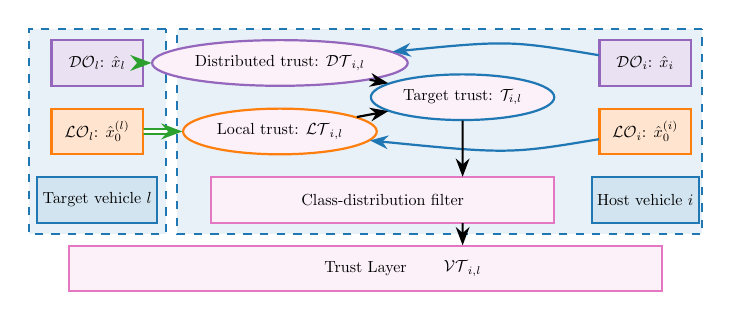
\begin{tikzpicture}[global scale = 0.58,
    vehicle/.style={draw=blue1, fill=blue1!20, thick, minimum width=2cm, minimum height=1cm},
    localobs/.style={draw=orange1, fill=orange1!20, thick, minimum width=2cm, minimum height=1cm},
    distobs/.style={draw=purple1, fill=purple1!20, thick, minimum width=2cm, minimum height=1cm},
    sigarrow/.style={-Stealth, thick, color=blue1},
    commarrow/.style={
    double,
    double distance=1pt,
    line width=0.7pt,
    draw=green1,
    -Stealth
    },
    physics/.style={draw=blue1, shape=rectangle, fill=blue1!10,line width=0.75pt,dashed,minimum width=3cm, minimum height=4.5cm}, %
    trustlayer/.style={draw=rose1, shape=rectangle, fill=rose1!10,thick,minimum width=13cm, minimum height=1cm},
    trust/.style={draw=rose1, shape=ellipse, fill=rose1!10,thick,minimum width=1.5cm, minimum height=1cm}
]

        \node[physics,line width=0.75pt,minimum width=3cm, minimum height=4.5cm] at(2,1.5) { };
        \node[vehicle, name=target] at(2,0) {Target vehicle $l$};
        \node[localobs, name=LOt] at(2,1.5) {$\LO_{l}$: $\hat{x}_{0}^{(l)}$};
        \node[distobs, name=DOt] at(2,3) {$\DO_{l}$: $\hat{x}_{l}$};

        \node[physics,line width=0.75pt,minimum width=11.5cm, minimum height=4.5cm,name=host] at(9.5,1.5) {};
        \node[vehicle,name=host] at(14,0) {Host vehicle $i$};
        \node[localobs,name=LOh] at(14,1.5) {$\LO_{i}$: $\hat{x}_{0}^{(i)}$};
        \node[distobs,name=DOh] at(14,3) {$\DO_{i}$: $\hat{x}_{i}$};

        \node[trust,draw = purple1, name=DT] at(6,3) {Distributed trust: $\DT_{i,l}$};
        \node[trust,draw = orange1, name=LT] at(6,1.5) {Local trust:  $\LT_{i,l}$};
        \node[trust,draw = blue1, name=T] at(10,2.25) {Target trust: $\T_{i,l}$};

        \node[trust,shape=rectangle,name=evo, minimum width=7.5cm] at(8.25,0) {Class-distribution filter};
        \node[name=evo,minimum height=1cm] at(10,0) {};

        \node[trustlayer] at(0.5/2+15.25/2,-1.5) {Trust Layer};
        \node[name = VT,minimum height=1cm] at(10,-1.5) {$\VT_{i,l}$};

        \draw[commarrow] (DOt) -- (DT);
        \draw[commarrow] (LOt) -- (LT);

        \draw[sigarrow] (LOh) .. controls +(-3,-0.5).. (LT);
        \draw[sigarrow] (DOh) .. controls +(-3,0.5).. (DT);

        \draw[sigarrow, black] (LT) -- (T);
        \draw[sigarrow,black] (DT) -- (T);

        \draw[sigarrow,black] (T) -- (evo);
        \draw[sigarrow,black] (evo) -- (VT);
    \end{tikzpicture}
    \caption{Trust framework.}
    \label{fig_trust_framework}
\end{figure}

In this context, we define the following types of trust:
\begin{itemize}
    \item \textbf{Local Trust $\LT_{i,l}$}: reliability of vehicle $l$'s local-observer data.
    \item \textbf{Distributed Trust $\DT_{i,l}$}: agreement between distributed estimates from $l$ and those of $i$.
    \item \textbf{Target Trust $\T_{i,l}$}: instantaneous fusion of Local Trust and Distributed Trust.
    \item \textbf{Vehicle Trust $\VT_{i,l}$}: class-filtered trust score used by the observer.
\end{itemize}

The following subsections define these scores and their use in the observer.
\subsection{Data validity indicator}

Before trust computation, each received V2V packet is checked for authenticity and freshness:
{\small
\begin{equation}
    \delta_{i,l}(t)=
    \begin{cases}
        1, & \text{if the message is authenticated and fresh}, \\
        0, & \text{otherwise.}
    \end{cases}
\end{equation}
}
Only packets with $\delta_{i,l}(t)=1$ are used for trust evaluation.

\subsection{Local trust}\label{sub:local_trust}

Local Trust $\LT_{i,l}$ measures the confidence of host vehicle $i$ in the local-observer output of neighbor $l \in \N_i$.
It uses bicycle-state consistency indicators: planar position, speed, heading, and an optional input-consistency check for acceleration and steering. Missing data are handled by a hold-and-decay rule.

\subsubsection{Planar position consistency}
Let $p_i=[X_i,Y_i]^\top$. The host transforms its onboard relative measurement of vehicle $l$ into the global frame and denotes it by $r_{i,l}^{\mathrm{meas}}(t)\in\mathbb{R}^2$. The relative position implied by the local observers is
\begin{equation*}
    r_{i,l}^{\mathrm{obs}}(t)=
    \begin{bmatrix}\hat X_0^{(l)}(t)-\hat X_0^{(i)}(t)\\
    \hat Y_0^{(l)}(t)-\hat Y_0^{(i)}(t)
    \end{bmatrix}.
\end{equation*}
The position-consistency score is
\begin{equation*}
    \iota_{i,l}^{\text{pos}}
    =
    \max\left(
    1 -
    \frac{\left\|r_{i,l}^{\mathrm{obs}}-r_{i,l}^{\mathrm{meas}}\right\|}
    {\varepsilon_p+\left\|r_{i,l}^{\mathrm{meas}}\right\|},
    0
    \right),
\end{equation*}
where $\varepsilon_p>0$ avoids division by zero.

\subsubsection{Speed consistency}
The host compares the relative speed implied by the two local observers with the onboard measured relative speed $v_{i,l}^{\mathrm{rel,meas}}(t)$:
\begin{equation*}
    \iota_{i,l}^{\text{speed}}
    =
    \max\left(
    1 -
    \frac{\left|(\hat{v}_{0}^{(l)}-\hat{v}_{0}^{(i)})-v_{i,l}^{\mathrm{rel,meas}}\right|}
    {\varepsilon_v+\left|v_{i,l}^{\mathrm{rel,meas}}\right|},
    0
    \right),
\end{equation*}
where $\varepsilon_v>0$ avoids division by zero.

\subsubsection{Heading consistency}
Heading is checked using the reported yaw and a motion-derived yaw estimate. From two consecutive accepted position reports from vehicle $l$,
\begin{equation*}
    \psi_{l}^{\mathrm{pos}}(t)=
    \mathrm{atan2}\big(\hat Y_0^{(l)}(t)-\hat Y_0^{(l)}(t-1),
    \hat X_0^{(l)}(t)-\hat X_0^{(l)}(t-1)\big).
\end{equation*}
If radar azimuth or LiDAR shape orientation is available, it can replace or complement $\psi_l^{\mathrm{pos}}(t)$. The heading score is
\begin{equation*}
    \iota_{i,l}^{\text{heading}} =
    \max\left(
    1-\frac{\left|\mathrm{wrap}_{\pi}(\hat{\psi}_0^{(l)}-\psi_l^{\mathrm{pos}})\right|}
    {\varepsilon_{\psi}+\psi_{\mathrm{th}}},
    0
    \right),
\end{equation*}
where $\psi_{\mathrm{th}}>0$ is a nominal heading tolerance. This check implements the heading-verification mechanism based on consecutive position reports or bearing measurements.
\begin{assumption}\label{assum_connect}
When a vehicle is connected, it has access to basic information about its neighbors, including their type, length, and nominal wheelbase class.
\end{assumption}

\subsubsection{Optional input consistency}
If acceleration and steering commands are included in the received packet, the host checks them against finite-difference speed and yaw-rate estimates:
\begin{align*}
    a_{l}^{\mathrm{fd}}(t)
    &=\frac{\hat v_0^{(l)}(t)-\hat v_0^{(l)}(t-n)}{nT_s},\\
    \omega_l^{\mathrm{bike}}(t)
    &=\frac{\hat v_0^{(l)}(t)}{L_w}\tan\hat\delta_l(t).
\end{align*}
With $\omega_l^{\mathrm{fd}}(t)=\mathrm{wrap}_{\pi}(\hat\psi_0^{(l)}(t)-\hat\psi_0^{(l)}(t-n))/(nT_s)$,
\begin{equation*}
    \iota_{i,l}^{\text{input}} =
    \max\left(
    1 -
    \frac{|\hat a_l-a_l^{\mathrm{fd}}|+|\omega_l^{\mathrm{bike}}-\omega_l^{\mathrm{fd}}|}
    {\varepsilon_u+a_{\mathrm{th}}+\omega_{\mathrm{th}}},
    0
    \right),
\end{equation*}
where $a_{\mathrm{th}}$ and $\omega_{\mathrm{th}}$ are nominal acceleration and yaw-rate tolerances. If the command channels are not transmitted, $\iota_{i,l}^{\text{input}}$ is omitted from the fusion.

\subsubsection{Fusion and update rule}
For simplicity and reproducibility, the available indicators are fused by a weighted geometric product. Let $\omega_p,\omega_v,\omega_\psi,\omega_u\ge0$ denote channel exponents. When the input channel is available, the local trust score is
\begin{align}
    \LT_{i,l}^{\mathrm{raw}}(t)
    &=\left(\iota_{i,l}^{\text{pos}}(t)\right)^{\omega_p}
    \left(\iota_{i,l}^{\text{speed}}(t)\right)^{\omega_v}
    \notag\\
    &\quad\times
    \left(\iota_{i,l}^{\text{heading}}(t)\right)^{\omega_\psi}
    \left(\iota_{i,l}^{\text{input}}(t)\right)^{\omega_u}.
    \label{eq_local_trust_product}
\end{align}
If the optional input channel is unavailable, the last factor is omitted. Missing or invalid packets are handled by
\begin{equation}
    \LT_{i,l}(t) =
    \left\{ \begin{array}{lc}
        \LT_{i,l}^{\mathrm{raw}}(t),  &  \text{if } \delta_{i,l}(t) = 1, \\
        (1 - \lambda_h)\LT_{i,l}(t-1), & \text{otherwise}
    \end{array}\right.
    \label{eq_local_trust_update}
\end{equation}
where $\lambda_h$ sets the decay rate during data loss.
\begin{remark}
    Multiplicative fusion is conservative: one inconsistent channel is enough to reduce the local trust score. Larger exponents assign stronger influence to the corresponding consistency channel. The decay $\lambda_h$ can increase with consecutive missed packets.
\end{remark}

\subsection{Distributed trust}
Distributed Trust applies the same idea to exchanged distributed estimates. It is defined as
\begin{equation}
        \DT_{i,l}(t)  = \begin{cases}
       \gamma_{i,l}^{\text{self}}(t) \cdot \gamma_{i,l}^{\text{local}}(t) \cdot
        \gamma_{i,l}^{\text{host}}(t)   &  \text{if } \delta_{i,l}(t) = 1 \\
        (1 - \lambda_h)\DT_{i,l}(t-1), & \text{otherwise} \\
    \end{cases}
\end{equation}
where $\gamma_{i,l}^{\text{self}}$, $\gamma_{i,l}^{\text{host}}$, and $\gamma_{i,l}^{\text{local}}$ check consistency with the sender's local observer, the host's distributed estimate, and the host's local measurements, respectively.

\subsubsection{Sender self-consistency}
The sender's distributed estimate of its own state should remain close to its local observer state:
\begin{equation}
    \begin{aligned}
    \gamma_{i,l}^{\text{self}}(t)
    &=
    \exp\Big(
    -(\hat{x}_l^{(l)}(t)-\hat{x}_0^{(l)}(t))^{\top}
    \Sigma_{\text{self}}^{-1} \\
    &\qquad\quad \times
    (\hat{x}_l^{(l)}(t)-\hat{x}_0^{(l)}(t))
    \Big),
    \end{aligned}
\end{equation}
where $\Sigma_{\text{self}}$ is the covariance matrix associated with the sender self-consistency residual.

\subsubsection{Host-estimate consistency}
The host compares the estimate received from target $l$ with its own estimate using the Mahalanobis distance:
\begin{equation}
    \rho_{i,l}^{(j)}(t) = \left( \hat{x}_i^{(j)}(t) - \hat{x}_l^{(j)}(t) \right)^{\top} \Sigma_{\text{host}}^{-1} \left( \hat{x}_i^{(j)}(t) - \hat{x}_l^{(j)}(t) \right)
    \label{eq_dis_glo}
\end{equation}
where $\Sigma_{\text{host}}$ is the diagonal covariance matrix of state-channel discrepancies:
\begin{equation}
\Sigma_{\text{host}} = \diag{\sigma^2_1, \sigma^2_2, \cdots , \sigma^2_n},
\end{equation}
where $n$ is the number of states and $\sigma^2_k$ is the variance of the $k$th state discrepancy.

The total discrepancy score is
\begin{equation}
    D_{i,l}^{\text{host}}(t) = \sum_{j=1}^N \rho_{i,l}^{(j)}(t).
\end{equation}
A small $D_{i,l}^{\text{host}}(t)$ means that vehicle $l$'s estimates are close to the host's estimates. The corresponding trust factor is
\begin{equation}
    \gamma_{i,l}^{\text{host}}(t) = \exp\left( -D_{i,l}^{\text{host}}(t) \right).
\end{equation}
where $\gamma_{i,l}^{\text{host}}(t) \in (0, 1]$.

\subsubsection{Consistency with host's local measurement}
Host vehicle $i$ uses relative measurements to nearby vehicles, e.g., planar relative position, range, bearing, relative speed, or heading difference, to check whether the estimates from target $l$ are consistent with local sensing.

Let $y_{i,j}(t) \in \mathbb{R}^{m_{ij}}$ be the relative measurement from vehicle $i$ to vehicle $j$, e.g., the global-frame relative position $p_j(t)-p_i(t)$ or a range-bearing vector transformed through the host pose.

The estimate received from target $l$ should approximately satisfy
\begin{equation*}
    H(\hat{x}_l^{(j)}(t) - \hat{x}_l^{(i)}(t)) \approx y_{i,j}(t).
\end{equation*}
where $H \in \mathbb{R}^{m_{ij} \times n}$ extracts the measured states.

The consistency error is
\begin{equation}
    \varepsilon_{i,l}^{(j)}(t) = H\left( \hat{x}_l^{(j)}(t) - \hat{x}_l^{(i)}(t) \right) - y_{i,j}(t),
\end{equation}
Using $\Sigma_{\text{local}}$ as in~\eqref{eq_dis_glo}, define
\begin{equation}
    E_{i,l}^{(j)}(t) = (\varepsilon_{i,l}^{(j)}(t))^{\top} \Sigma_{\text{local}}^{-1} \varepsilon_{i,l}^{(j)}(t).
\end{equation}

The total consistency error is
\begin{equation}
    E_{i,l}(t) = \sum_{j \in \N_i} E_{i,l}^{(j)}(t).
\end{equation}
A higher $E_{i,l}(t)$ means that the estimates from target $l$ disagree with local relative measurements.

The trust factor is
\begin{equation}
    \gamma_{i,l}^{\text{local}}(t) = \exp\left( -{E_{i,l}(t)} \right),
\end{equation}
where $\gamma_{i,l}^{\text{local}}(t) \in (0, 1]$.
\begin{remark}
The covariance matrices $\Sigma_{\text{host}}$ and $\Sigma_{\text{local}}$ can be estimated from a recent nominal-data window at vehicle \(i\), avoiding covariance transmission between nodes.
\end{remark}
\subsection{Target trust and temporal evolution}\label{subsec_evolution}
We combine the Local Trust and Distributed Trust into a single instantaneous trust score for target $l$:
\begin{equation}
    \T_{i,l}(t) =  \LT_{i,l}(t) \cdot \DT_{i,l}(t).
    \label{trs_sample_genral}
\end{equation}
$\T_{i,l}(t)$ measures the instantaneous quality of target $l$'s data.
Because this value can vary abruptly, a class-distribution temporal filter is used instead of applying the instantaneous scalar directly.
Let $q=5$ denote the number of ordered trust classes:
\textit{Unreliable}, \textit{Poor}, \textit{Acceptable}, \textit{Good}, and \textit{Excellent}.
Define the class scores
\begin{equation}
    \rho_m=\frac{m-1}{q-1}, \qquad m=1,\ldots,q,
\end{equation}
and the corresponding intervals
\begin{equation}
    \mathcal{I}_m =
    \begin{cases}
    \left[\dfrac{m-1}{q},\dfrac{m}{q}\right), & m=1,\ldots,q-1,\\[1ex]
    \left[\dfrac{q-1}{q},1\right], & m=q.
    \end{cases}
\end{equation}
The instantaneous trust value is discretized into a one-hot class vector
\begin{equation}
    r_{i,l,m}(t)=
    \begin{cases}
    1, & \T_{i,l}(t)\in \mathcal{I}_m,\\
    0, & \text{otherwise,}
    \end{cases}
    \qquad
    r_{i,l}(t)\in\mathbb{R}^{q}.
\end{equation}
For example, $\T_{i,l}(t)=0.72$ belongs to the \textit{Good} class for $q=5$, so $r_{i,l}(t)=[0,0,0,1,0]^\top$.

The accumulated class evidence is updated as
\begin{equation}
    R_{i,l}(t+1)=
    \left(1-\beta_{\text{trust}}\T_{i,l}(t)\right)R_{i,l}(t)
    +r_{i,l}(t),
    \label{eq_class_history_update}
\end{equation}
where $R_{i,l}(t)\in\mathbb{R}_{\ge0}^{q}$ is initialized as $R_{i,l}(0)=0$ unless prior interaction evidence is available, and $\beta_{\text{trust}}\in[0,1]$ controls the decay of past class evidence.
The modulation by $\T_{i,l}(t)$ prevents one isolated low-quality sample from immediately erasing the accumulated history, while repeated low-quality samples keep adding evidence to the lower classes.
To regularize the class distribution, let $\alpha_{\mathrm{tr}}\in\mathbb{R}_{\ge0}^{q}$ be a prior trust-class distribution satisfying $\sum_{m=1}^{q}\alpha_{\mathrm{tr},m}=1$, and let $C_{\mathrm{tr}}>0$ be a confidence parameter.
The prior $\alpha_{\mathrm{tr}}$ represents the initial belief about vehicle $l$ before enough packets are observed; if no prior information is available, one can use the uniform choice $\alpha_{\mathrm{tr},m}=1/q$.
The parameter $C_{\mathrm{tr}}$ controls how strongly this prior affects the estimate: larger $C_{\mathrm{tr}}$ gives more weight to the prior, while smaller $C_{\mathrm{tr}}$ lets online evidence dominate faster.
The normalized trust-class distribution is
\begin{equation}
    S_{i,l,m}(t)=
    \frac{R_{i,l,m}(t)+C_{\mathrm{tr}}\alpha_{\mathrm{tr},m}}
    {C_{\mathrm{tr}}+\sum_{s=1}^{q}R_{i,l,s}(t)},
    \qquad m=1,\ldots,q.
    \label{eq_class_distribution}
\end{equation}
The smoothed vehicle trust used by the observer is the expected trust level
\begin{equation}
    \VT_{i,l}(t)=
    \sum_{m=1}^{q}\rho_m S_{i,l,m}(t).
    \label{eq_class_filtered_vehicle_trust}
\end{equation}
A larger $\beta_{\text{trust}}$ gives a more reactive trust history, while a smaller value gives smoother trust evolution.
The confidence $C_{\mathrm{tr}}$ controls how strongly the prior influences the estimate when only a short interaction history is available.
The observer uses $\VT_{i,l}(t)$ to weigh information received from vehicle $l$.

\subsection{Practical parameter selection}\label{subsec_trust_tuning}
The trust parameters are selected from nominal data and physical limits rather than tuned directly on attack cases. First, the receiver defines the admissible packet set $\Omega_z$ in~\eqref{eq_received_packet_gate} from vehicle limits, road geometry, timestamp tolerance, maximum speed, acceleration, steering angle, and feasible inter-sample motion. Second, the covariance matrices $\Sigma_{\text{self}}$, $\Sigma_{\text{host}}$, and $\Sigma_{\text{local}}$ are estimated from an attack-free calibration window and regularized with positive lower bounds on every diagonal entry. Third, the exponents $\omega_p,\omega_v,\omega_\psi,\omega_u$ encode channel confidence: a channel with lower nominal noise or higher safety relevance receives a larger exponent, while an unavailable channel is removed from the product. Fourth, the threshold $\theta_{\min}$ is chosen from nominal validation data so that benign packets are rarely rejected, then checked under representative faults. Finally, $\beta_{\text{trust}}$ and $C_{\mathrm{tr}}$ set the detection--recovery tradeoff: larger $\beta_{\text{trust}}$ reacts faster to repeated low-trust evidence, while larger $C_{\mathrm{tr}}$ prevents short histories from dominating the prior. After these values are fixed, the observer weights are checked against the stability conditions in Section~\ref{sec_weight_design}.


% For the controller interface, each host vehicle also forms an opinion vector
% \begin{equation}
%     \O_i(t)=[\O_i(1,t),\ldots,\O_i(N,t)],
% \end{equation}
% where $\O_i(i,t)=1$ and $\O_i(l,t)=\VT_{i,l}(t)$ for trusted neighbors. For non-neighboring vehicles, $\O_i(j,t)$ can be obtained from one-hop propagated opinions or assigned a conservative default when no credible propagated opinion is available. This vector is used only as a compact reliability summary for the controller blending factor in Section~\ref{sec_simulation}; the observer-weight design below uses the pairwise trust values directly.

\section{Trust-Based Observer Weight Design}\label{sec_weight_design}
The trust framework provides each vehicle with smoothed vehicle-trust scores $\VT_{i,l}(t)$ representing the reliability of information from other vehicles.
This section shows how these values are used to define adaptive observer weights $w_{il}^{(j)}(t)$ and establishes conditions for stability of the estimation error dynamics.

\subsection{Weight based on the trust}
Using the virtual graph $\bar{\G}^{(j)}$, each vehicle $i$ first selects the trusted neighbor sources at time $t$:
\begin{equation}
\mathcal{LN}^{(j)}_{i}(t)
= \Big\{\, l \in \N_i \;\big|\; \VT_{i,l}(t) \ge \theta_{\min} \Big\}.
\end{equation}
The selected trust scores are then used directly as reliability scores,
\begin{align}
s_{i,l}^{(j)}(t)
&=
\begin{cases}
\VT_{i,l}(t), & l\in\mathcal{LN}^{(j)}_{i}(t),\\
0, & \text{otherwise},
\end{cases}
\label{new_setneibor}\\
S_i^{(j)}(t)
&=\epsilon+\sum_{r\in\N_i}s_{i,r}^{(j)}(t),
\end{align}
where $\epsilon>0$ avoids division by zero. Let $\eta_0,\eta_N\in[0,1]$ denote the local-anchor and neighbor-consensus budgets, respectively, with
\begin{equation}
    \eta_0+\eta_N\le1 .
\end{equation}
Let $\chi_{i0}^{(j)}(t)\in\{0,1\}$ indicate that the local-anchor packet $\hat{x}_0^{(j)}(t)$ is available and accepted at host $i$. For the target's own host, $\chi_{j0}^{(j)}(t)=1$ and $\LT_{j,j}(t)=1$; if the anchor packet is unavailable or rejected, $\chi_{i0}^{(j)}(t)=0$ and the anchor weight is zero. The local-anchor weight is
\begin{equation}\label{eq_anchor_weight}
w_{i0}^{(j)}(t)=
\begin{cases}
\eta_0\chi_{i0}^{(j)}(t)\LT_{i,j}(t), &
\substack{\chi_{i0}^{(j)}(t)=1,\\ \LT_{i,j}(t)\ge\theta_{\min},}\\
0, & \text{otherwise},
\end{cases}
\end{equation}
and the neighbor weights are
\begin{equation}\label{design_gain}
    w_{il}^{(j)}(t)
    =
    \eta_N
    \frac{s_{i,l}^{(j)}(t)}
    {S_i^{(j)}(t)},
    \qquad l\in\N_i .
\end{equation}
Thus, rejected neighbors receive zero weight, while accepted neighbors share the fixed budget $\eta_N$ in proportion to their trust values. The remaining mass is the implicit self-prediction weight
\begin{equation}
    w_{is}^{(j)}(t)
    =
    1-w_{i0}^{(j)}(t)-\sum_{l\in\N_i}w_{il}^{(j)}(t).
\end{equation}

The following lemma shows that the proposed trust-based weight law always
generates admissible mixing coefficients. In particular, the correction step
is a nonnegative weighted combination of the self prediction, trusted neighbors,
and the local-observer anchor. This property is important because it prevents
the observer from extrapolating unreliable information and guarantees that
bounded attacks enter the error dynamics only through bounded weighted inputs.

\begin{lemma}[Admissibility of trust weights]\label{lem_weight_admissible}
The weight law~\eqref{new_setneibor}--\eqref{design_gain} satisfies $w_{il}^{(j)}(t)\ge0$, $w_{i0}^{(j)}(t)\ge0$, and
\begin{equation}
\sum_{l\in\N_i\cup\{0\}}w_{il}^{(j)}(t)\le1
\end{equation}
for all $i,j$ and all $t$.
\end{lemma}
\begin{proof}
By construction, $s_{i,l}^{(j)}(t)\ge0$ and $S_i^{(j)}(t)>0$, hence $w_{il}^{(j)}(t)\ge0$ for all $l\in\N_i$. Also, $0\le w_{i0}^{(j)}(t)\le \eta_0$ because $\chi_{i0}^{(j)}(t)\in\{0,1\}$ and $\LT_{i,j}(t)\in[0,1]$. The neighbor contribution satisfies
\begin{align*}
\sum_{l\in\N_i}w_{il}^{(j)}(t)
&=
\eta_N
\frac{\sum_{l\in\N_i}s_{i,l}^{(j)}(t)}
{\epsilon+\sum_{l\in\N_i}s_{i,l}^{(j)}(t)}
\le \eta_N .
\end{align*}
Therefore,
\[
\sum_{l\in\N_i\cup\{0\}}w_{il}^{(j)}(t)
=w_{i0}^{(j)}(t)+\sum_{l\in\N_i}w_{il}^{(j)}(t)
\le \eta_0+\eta_N\le1 .
\]
\end{proof}

The lemma provides bounded mixing, but bounded mixing alone is not sufficient for convergence because the bicycle model contains prediction dynamics. The accepted trust-induced weights must also provide enough local-anchor mass, or enough rooted multi-step information flow, to contract the distributed prediction error. Let
\begin{equation}
    M^{(j)}(t)=I_N-\bar{\L}^{(j)}(t).
\end{equation}
By Lemma~\ref{lem_weight_admissible}, $M^{(j)}(t)$ is nonnegative and its $i$th row sum is $1-w_{i0}^{(j)}(t)$. Therefore, in the infinity norm,
\begin{equation}
    \|M^{(j)}(t)\|_{\infty}
    =
    \max_{i\in\V}\big(1-w_{i0}^{(j)}(t)\big).
    \label{eq_M_inf_norm}
\end{equation}
The proposed weight law gives a direct lower bound on this missing row mass whenever the target-local anchor packet is accepted.

\begin{lemma}[Anchor-induced one-step contraction]\label{lem_anchor_contraction}
Suppose that, for target $j$, the accepted anchor packet is available to every host at time $t$ and satisfies $\chi_{i0}^{(j)}(t)=1$ and $\LT_{i,j}(t)\ge\theta_{\min}$ for all $i\in\V$. Then the weight law~\eqref{eq_anchor_weight} gives
\begin{equation}
    w_{i0}^{(j)}(t)\ge \underline w_0,
    \qquad
    \underline w_0:=\eta_0\theta_{\min} .
\end{equation}
Consequently,
\begin{equation}
    \|M^{(j)}(t)\|_{\infty}\le 1-\underline w_0.
\end{equation}
If the bicycle map is Lipschitz on the admissible compact region in the same state norm with constant $L_{x,j}$ and
\begin{equation}
    L_{x,j}\big(1-\underline w_0\big)<1,
    \label{eq_anchor_contraction_check}
\end{equation}
then the homogeneous distributed prediction error is a one-step contraction.
\end{lemma}
\begin{proof}
Under the stated acceptance condition,~\eqref{eq_anchor_weight} gives $w_{i0}^{(j)}(t)=\eta_0\LT_{i,j}(t)\ge\eta_0\theta_{\min}$. The row-sum identity~\eqref{eq_M_inf_norm} then gives $\|M^{(j)}(t)\|_{\infty}\le1-\underline w_0$. Combining this with~\eqref{eq_nonlinear_lipschitz} yields the contraction factor in~\eqref{eq_anchor_contraction_check}.
\end{proof}

When direct anchors are intermittent, the same argument must be applied over a window. These weights induce a switching communication graph because the trusted-neighbor set changes online. A plain union spanning tree is not enough unless the anchor information can move through the matrix product in time order. We therefore use the following sequential rooted accepted-graph condition, where an edge $l\to i$ means that the accepted weight $w_{il}^{(j)}$ is positive.
\begin{assumption}[Sequentially rooted accepted graph]\label{ass_graph}
There exist an integer $T_c>0$ and a scalar $\underline w>0$ such that, for every target $j$, every start time $t\ge0$, and every host $i\in\V$, there are nodes $v_0=0,v_1,\ldots,v_m=i$ and times $t\le \tau_1<\cdots<\tau_m\le t+T_c-1$ for which the accepted edge $v_{r-1}\to v_r$ is present in $\bar{\G}^{(j)}(\tau_r)$. Each accepted edge weight on these temporal paths is at least $\underline w$, and each implicit self-prediction weight used to carry information between two consecutive path times is also at least $\underline w$.
\end{assumption}
Assumption~\ref{ass_graph} means that every host estimate of target $j$ receives anchor information either directly or through trusted intermediate estimates within each window. This is stronger than ordinary connectivity: the root must be the target-local observer node, the links must be accepted by the trust layer, and the path must be ordered along the product. A standard jointly rooted union condition implies this assumption after enlarging the window when accepted links recur in every joint-connectivity interval and the implicit self-prediction weights are uniformly positive; otherwise the product condition below must be verified directly.

\begin{lemma}[Rooted block contraction]\label{lem_rooted_block_contraction}
If Assumption~\ref{ass_graph} holds, then the grounded trust-mixing product satisfies
\begin{equation}
    \left\|
    M^{(j)}(t+T_c-1)\cdots M^{(j)}(t)
    \right\|_{\infty}
    \le 1-\underline w^{T_c} .
    \label{eq_grounded_product_bound}
\end{equation}
Let $G_{x,j}(T_c)$ be an upper bound, in the chosen state norm, on the nonlinear bicycle prediction gain over any admissible $T_c$-step block. If
\begin{equation}
    G_{x,j}(T_c)\big(1-\underline w^{T_c}\big)
    \le \alpha_c<1,
    \label{eq_window_contraction_check}
\end{equation}
then the distributed homogeneous error is contractive over every window of length $T_c$. The one-step condition~\eqref{eq_anchor_contraction_check} is the special case $T_c=1$ with direct anchor acceptance at every step.
\end{lemma}
\begin{proof}
The matrices $M^{(j)}(\tau)$ are nonnegative and substochastic. A positive anchor weight creates a strict row-sum deficit in the row receiving that anchor. For any host $i$, Assumption~\ref{ass_graph} gives a temporal accepted path from the anchor to $i$. Each accepted edge transmits at least a factor $\underline w$ of the existing deficit to the next node, and each waiting step preserves at least a factor $\underline w$ through the implicit self-prediction weight. Since the path transmissions and waiting steps occupy no more than $T_c$ time instants, the $i$th row sum of $M^{(j)}(t+T_c-1)\cdots M^{(j)}(t)$ is at most $1-\underline w^{T_c}$. Taking the maximum row sum gives~\eqref{eq_grounded_product_bound}. Multiplying by the bounded $T_c$-step bicycle prediction gain gives~\eqref{eq_window_contraction_check}.
\end{proof}

Thus, contraction is not assumed from trust scoring alone. The weight law supplies the anchor lower bound through $\eta_0\theta_{\min}$ when anchor packets are directly accepted, and Assumption~\ref{ass_graph} supplies the corresponding lower bound for sparse or intermittent trusted paths. If all reliable paths to a target are rejected, the theorem applies only to the reachable part of the platoon, and that target cannot be reconstructed from communication alone.

\subsection{Observer design procedure}
The complete design can be implemented through the following steps.
\begin{enumerate}
    \item Select a compact operating region $\Omega_x\times\Omega_u$ from vehicle limits and the receiving-side gate~\eqref{eq_received_packet_gate}. Compute conservative bounds for the bicycle Lipschitz constants $L_{x,j}$ and $L_{u,j}$ on this region.
    \item Choose the local observer gain $F_j(t)$ so that the zero-input local error recursion is uniformly locally exponentially stable. With full-state local measurements, this can be checked directly from the local linearization $A_j(t)-F_j(t)C_j(t)$ along the considered trajectory.
    \item Fix the trust parameters using the nominal-data procedure in Section~\ref{subsec_trust_tuning}, then compute $\VT_{i,l}(t)$, $\LT_{i,j}(t)$, and the acceptance variables $\delta_{i,l}(t)$ and $\chi_{i0}^{(j)}(t)$ online.
    \item Compute the anchor and neighbor weights from~\eqref{eq_anchor_weight}--\eqref{design_gain}. Lemma~\ref{lem_weight_admissible} guarantees that the resulting correction is a nonnegative bounded mixture.
    \item Check the contraction condition~\eqref{eq_anchor_contraction_check} or~\eqref{eq_window_contraction_check}. If the check fails for a target, the implementation should increase the anchor budget when a reliable anchor exists, reduce neighbor reliance, hold the last trusted estimate, or mark the target temporarily unreachable rather than injecting unverified cooperative data.
\end{enumerate}

\subsection{Stability of the error}\label{subsec_Prove}
We first write the estimation errors induced directly by the nonlinear observer in Section~\ref{sec_distributed_observer}. For a fixed target vehicle $j\in\V$, define the local-observer error and the distributed-observer errors in local state-difference coordinates as
\begin{equation}\label{eq:def_nonlinear_errors}
\begin{aligned}
e_0^{(j)}(t)&\triangleq \hat{x}_0^{(j)}(t)-x_j(t),\\
e_i^{(j)}(t)&\triangleq \hat{x}_i^{(j)}(t)-x_j(t),\quad i\in\V,
\end{aligned}
\end{equation}
and stack
\begin{equation}\label{eq:def_eDO}
e_{\DO}^{(j)}(t)=\col{e_1^{(j)}(t),\cdots,e_N^{(j)}(t)} .
\end{equation}
Using~\eqref{eq_LO} and the nonlinear plant dynamics, the original local-observer error recursion is
\begin{align}
e_0^{(j)}(t+1)
&=\Big[
f_{\mathrm{b}}\big(\hat{x}_0^{(j)}(t),u_j(t)\big)
 \notag\\
&\quad+F_j(t)\Big(y_j(t)-h_j\big(\hat{x}_0^{(j)}(t)\big)\Big)
\Big]\notag\\
&\quad -
\Big[
f_{\mathrm{b}}\big(x_j(t),u_j(t)\big)+\Delta_j(t)
\Big].
\label{eq_raw_e0}
\end{align}
Similarly, using~\eqref{eq_consensus_state}--\eqref{eq_DO}, each distributed-observer error satisfies the nonlinear recursion
\begin{align}
e_i^{(j)}(t+1)
&=f_{\mathrm{b}}\big(\hat{x}_{i,c}^{(j)}(t),\hat{u}_j(t)\big)\notag\\
&\quad -
\Big[
f_{\mathrm{b}}\big(x_j(t),u_j(t)\big)+\Delta_j(t)
\Big],
\label{eq_raw_ei}
\end{align}
where
\begin{align}
\hat{x}_{i,c}^{(j)}(t)
&= \hat{x}_i^{(j)}(t)
+\sum_{l \in \N_i} w_{il}^{(j)}(t)
   \big(\hat{x}_l^{(j)}(t)-\hat{x}_i^{(j)}(t)\big)\notag\\
&\quad + w_{i0}^{(j)}(t)
   \big(\hat{x}_0^{(j)}(t)-\hat{x}_i^{(j)}(t)\big).
\label{eq_raw_consensus_state}
\end{align}
Equivalently, the stacked nonlinear distributed-error dynamics are
\begin{equation}\label{eq_raw_eDO}
e_{\DO}^{(j)}(t+1)
=
\begin{bmatrix}
    f_{\mathrm{b}}\big(\hat{x}_{1,c}^{(j)}(t),\hat{u}_j(t)\big)-x_j(t+1) \\
    \vdots \\
    f_{\mathrm{b}}\big(\hat{x}_{N,c}^{(j)}(t),\hat{u}_j(t)\big)-x_j(t+1)
    \end{bmatrix}
\end{equation}
Equations~\eqref{eq_raw_e0}--\eqref{eq_raw_eDO} are the original nonlinear error dynamics used in the ISS analysis. The result is local on a compact operating region $\Omega_x\times\Omega_u$ containing the considered trajectories, with bounded speed, bounded inputs, no yaw-chart discontinuity, and $|\delta|\le \delta_{\max}<\pi/2$. On this region the bicycle map is locally Lipschitz: there exist finite constants $L_{x,j}>0$ and $L_{u,j}>0$ such that
\begin{equation}
\begin{aligned}
\|f_{\mathrm b}(\xi,\mu)-f_{\mathrm b}(\zeta,\nu)\|_*
&\le L_{x,j}\|\xi-\zeta\|_*\\
&\quad+L_{u,j}\|\mu-\nu\|_*
\end{aligned}
\label{eq_nonlinear_lipschitz}
\end{equation}
for all $(\xi,\mu),(\zeta,\nu)\in\Omega_x\times\Omega_u$. The Jacobian model below is therefore used to compute conservative bounds and to synthesize $F_j(t)$, while the theorem is stated for the nonlinear recursions~\eqref{eq_raw_e0}--\eqref{eq_raw_eDO}.


Let $\bar{x}_j(t)=\col{\bar X_j(t),\bar Y_j(t),\bar\psi_j(t),\bar v_j(t)}$ and
$\bar u_j(t)=\col{\bar a_j(t),\bar\delta_j(t)}$ be the trajectory about which the
nonlinear bicycle model is linearized. The Jacobians used to obtain conservative
local values of $L_{x,j}$ and $L_{u,j}$, and to check the local-observer gain, are
\begin{align}
    A_i(t)&=\left.\frac{\partial f_{\text{b}}}{\partial x}\right|_{(\bar{x}_i(t),\bar{u}_i(t))},&
    B_i(t)&=\left.\frac{\partial f_{\text{b}}}{\partial u}\right|_{(\bar{x}_i(t),\bar{u}_i(t))},\notag\\
    C_i(t)&=\left.\frac{\partial h_i}{\partial x}\right|_{\bar{x}_i(t)}  = I_4.\notag
\end{align}
where
\begin{align}
A_i(t)=
\begin{bmatrix}
1&0&-T_s\bar v_i\sin\bar\psi_i&T_s\cos\bar\psi_i\\
0&1&T_s\bar v_i\cos\bar\psi_i&T_s\sin\bar\psi_i\\
0&0&1&\dfrac{T_s}{L_w}\tan\bar\delta_i\\
0&0&0&1
\end{bmatrix},
\label{eq_bicycle_jacobian}\\
B_i(t)=
\begin{bmatrix}
0&0\\
0&0\\
0&\dfrac{T_s\bar v_i}{L_w}\sec^2\bar\delta_i\\
T_s&0
\end{bmatrix}.
\notag
\end{align}

In the local state-difference coordinates, the correction step satisfies
\begin{equation}
    \begin{aligned}
\hat{x}_{i,c}^{(j)}(t)-x_j(t)
=&
\Big(1-w_{i0}^{(j)}(t)-\sum_{l\in\N_i}w_{il}^{(j)}(t)\Big)e_i^{(j)}(t)\\
&+
\sum_{l\in\N_i}w_{il}^{(j)}(t)e_l^{(j)}(t)\\
&+w_{i0}^{(j)}(t)e_0^{(j)}(t)+\rho_i^{(j)}(t),
    \end{aligned}
\label{eq:dominant_consensus_error}
\end{equation}
where $\rho_i^{(j)}(t)$ collects only the higher-order terms caused by a nonlinear
local-coordinate representation. Under the local no-wrap Euclidean chart used by
the bicycle state definition, this term is zero for the consensus algebra; for a
general local retraction, it is a bounded second-order remainder. Therefore,
using nonnegative weights with row sum not larger than one, the pre-prediction correction obeys
\begin{align}
\|\hat{x}_{i,c}^{(j)}(t)-x_j(t)\|_*
&\le
\Big(1-w_{i0}^{(j)}(t)-\sum_{l\in\N_i}w_{il}^{(j)}(t)\Big)
\|e_i^{(j)}(t)\|_* \notag\\
&\quad+
\sum_{l\in\N_i}w_{il}^{(j)}(t)\|e_l^{(j)}(t)\|_* \notag\\
&\quad+
w_{i0}^{(j)}(t)\|e_0^{(j)}(t)\|_* \notag\\
&\quad+\|\rho_i^{(j)}(t)\|_* .
\label{eq_nonlinear_consensus_bound}
\end{align}

For gain synthesis and for comparison with the standard linear observer design,
the first-order expansion along $\bar{x}_j(t)$ gives the auxiliary model
\begin{equation}\label{eq_e0}
   e_0^{(j)}(t+1) = \left( A_j(t) - F_{j}(t) C_j(t)  \right) e_0^{(j)}(t) + d_0^{(j)}(t),
\end{equation}
{\small
    \begin{align}\label{eq_error}
        e_{\DO}^{(j)}(t+1) &= \left( w_{0}^{(j)}(t) \otimes A_j(t) \right) e_0^{(j)}(t)  \notag\\
        &+ \left( \left( I_{N} - \bar{\L}^{(j)}(t)  \right)  \otimes  A_j(t) \right) e_{\DO}^{(j)}(t) + d_{\DO}^{(j)}(t),
    \end{align}
}
with
\begin{align*}
    d_0^{(j)}(t) &= r_0^{(j)}(t)- \Delta_j(t), \\
    d_{\DO}^{(j)}(t)  &= (\mathbf{1}_N \otimes B_j(t))(\hat{u}_j(t)-u_j(t)) \\
    &\quad + r_{\DO}^{(j)}(t) - (\mathbf{1}_N \otimes \Delta_j(t)), 
\end{align*}
where $r_0^{(j)}$ and $r_{\DO}^{(j)}$ collect bounded local approximation terms, including the higher-order terms $\rho_i^{(j)}$ generated by the local-coordinate representation. The ISS result below is stated for the nonlinear recursions; the auxiliary model~\eqref{eq_e0}--\eqref{eq_error} is used to select gains and to check conservative contraction constants on $\Omega_x\times\Omega_u$. 

The attack contribution can be written explicitly in the same error system.
Suppose that a received channel is corrupted before the correction step.
For compact notation, the receiving-host index is suppressed and host vehicle $i$ receives
\begin{equation}
    \tilde{x}_{0}^{(j)}(t)=\hat{x}_{0}^{(j)}(t)+a_{0}^{(j)}(t),
    \qquad
    \tilde{x}_{l}^{(j)}(t)=\hat{x}_{l}^{(j)}(t)+a_{l}^{(j)}(t),
\end{equation}
where $a_{0}^{(j)}$ corrupts the local-anchor signal and $a_{l}^{(j)}$ corrupts the distributed estimate received from neighbor $l$.
Let $\mathcal{M}_{i}^{(j)}(t)\subseteq\N_i$ denote the attacked neighbor channels at host $i$; for unattacked, unavailable, or rejected channels, the corresponding attack vector is set to zero.
Then the corrupted correction step adds the pre-prediction perturbation
{\small
\begin{equation}
\chi_{\mathrm{att},i}^{(j)}(t)
=w_{i0}^{(j)}(t)a_{0}^{(j)}(t)
+\sum_{l\in\mathcal{M}_{i}^{(j)}(t)}w_{il}^{(j)}(t)a_{l}^{(j)}(t).
\label{eq_attack_input}
\end{equation}
}
By~\eqref{eq_nonlinear_lipschitz}, this perturbation enters the nonlinear error recursion as an additive ISS input bounded by
\begin{equation}
\|d_{\mathrm{att},i}^{(j)}(t)\|_*
\le L_{x,j}\|\chi_{\mathrm{att},i}^{(j)}(t)\|_* .
\label{eq_attack_lipschitz_bound}
\end{equation}
Stacking the row-wise terms gives
\begin{equation}
    d_{\mathrm{att}}^{(j)}(t)
    =\col{d_{\mathrm{att},1}^{(j)}(t),\ldots,d_{\mathrm{att},N}^{(j)}(t)}.
\end{equation}
At the auxiliary linearized level, substituting the corrupted signals into~\eqref{eq_DO} gives
{\small
\begin{align}
e_{\DO}^{(j)}(t+1)
&= \left( w_{0}^{(j)}(t) \otimes A_j(t) \right) e_0^{(j)}(t)  \notag\\
&\quad+ \left( \left( I_{N} - \bar{\L}^{(j)}(t)  \right)  \otimes  A_j(t) \right) e_{\DO}^{(j)}(t)
+\tilde d_{\DO}^{(j)}(t),
\label{eq_error_attacked}
\end{align}
}
with
{\small
\begin{equation}
    \tilde d_{\DO}^{(j)}(t)
    =d_{\DO}^{(j)}(t)+d_{\mathrm{att}}^{(j)}(t).
\end{equation}
}
Thus, in both the nonlinear ISS inequality and its auxiliary linearized model, the attack is handled as an input whose size is modulated by the trust weights.
If $\|a_{0}^{(j)}(t)\|_*\le \bar a_0$ and $\|a_{l}^{(j)}(t)\|_*\le \bar a_{\mathrm{N}}$ on $\mathcal{M}_{i}^{(j)}(t)$, then Lemma~\ref{lem_weight_admissible} gives
\begin{align}
\|d_{\mathrm{att},i}^{(j)}(t)\|_*
&\le L_{x,j}
\left(
w_{i0}^{(j)}(t)\bar a_0
+\sum_{l\in\mathcal{M}_{i}^{(j)}(t)}
w_{il}^{(j)}(t)\bar a_{\mathrm{N}}
\right) \notag\\
&\le \bar A_j \max\{\bar a_0,\bar a_{\mathrm{N}}\}.
\label{eq_attack_bound}
\end{align}
where $\bar A_j$ can be chosen as any finite upper bound on $L_{x,j}$ over the compact operating region. Consequently, for the stacked vector there exists a finite constant $\bar d_{\mathrm{att}}$ such that
\begin{equation}
    \|d_{\mathrm{att}}^{(j)}(t)\|\le \bar d_{\mathrm{att}}.
\end{equation}
When the trust layer rejects a corrupted channel, the associated weight becomes zero and its contribution in~\eqref{eq_attack_input} disappears.

For the nonlinear ISS proof, $d_0^{(j)}$ and $d_{\DO}^{(j)}$ denote the corresponding lumped inputs caused by model uncertainty, input mismatch, chart remainders, and bounded approximation terms. We assume these inputs and the additive attack contribution are bounded.
\begin{assumption}\label{assum_distur}
There exist $\bar{d}_{0} \geq 0$, $\bar{d}_{\DO} \geq 0$, and $\bar d_{\mathrm{att}}\ge0$ such that, for all $t\geq 0$,
\[
\|d_0^{(j)}(t)\| \le \bar{d}_{0},
\qquad
\|d_{\DO}^{(j)}(t)\| \le \bar{d}_{\DO},
\qquad
\|d_{\mathrm{att}}^{(j)}(t)\| \le \bar d_{\mathrm{att}}.
\]
Equivalently, the attacked distributed-error input satisfies
\[
    \|\tilde d_{\DO}^{(j)}(t)\|\le
    \bar{\tilde d}_{\DO}:=\bar d_{\DO}+\bar d_{\mathrm{att}}.
\]
\end{assumption}

\begin{lemma}[Local nonlinear observer ISS]\label{lem_local_iss}
Assume that, on the compact operating region $\Omega_x\times\Omega_u$, the disturbance-free local nonlinear error recursion associated with~\eqref{eq_raw_e0} is uniformly locally exponentially stable. Equivalently, there exist $c_{\ell}>0$ and $\lambda_{\ell}\in(0,1)$ such that the zero-input local error satisfies the corresponding exponential bound for all admissible trajectories in the region. If Assumption~\ref{assum_distur} holds and the perturbed trajectory remains in the same region, then the local-observer error is ISS with respect to $d_0^{(j)}$. In particular,
\begin{equation}
\|e_0^{(j)}(t)\|\le c_{\ell}\lambda_{\ell}^{t}\|e_0^{(j)}(0)\|
+\frac{c_{\ell}}{1-\lambda_{\ell}}\bar d_0 .
\end{equation}
A sufficient local check is the uniform exponential stability of the linearized matrix $A_j(t)-F_j(t)C_j(t)$ together with a sufficiently small invariant neighborhood.
\end{lemma}
\begin{proof}
The local nonlinear error map is locally Lipschitz in the error and in the bounded input $d_0^{(j)}$ on $\Omega_x\times\Omega_u$. Uniform local exponential stability of the zero-input recursion gives a transition bound $c_{\ell}\lambda_{\ell}^{t-k}$. Unrolling the perturbed recursion and using Assumption~\ref{assum_distur} gives the stated geometric ISS estimate. The final statement follows from the standard Lyapunov indirect argument for discrete-time nonlinear systems on a compact region.
\end{proof}


\begin{lemma}[Nonlinear distributed-error contraction]\label{lem_dist_contraction}
Suppose that the block contraction condition~\eqref{assume3} below holds. If the local-observer error is ISS and Assumption~\ref{assum_distur} holds, then the nonlinear distributed error~\eqref{eq_raw_eDO} is ISS with respect to $e_0^{(j)}$ and $d_{\DO}^{(j)}$. Under the additive attack model, the attacked distributed error is ISS with respect to $e_0^{(j)}$ and $\tilde d_{\DO}^{(j)}$.
\end{lemma}
\begin{proof}
Let $M^{(j)}(t)=I_N-\bar{\L}^{(j)}(t)$ and denote $E(t)=\|e_{\DO}^{(j)}(t)\|_*$. Combining the nonlinear Lipschitz bound~\eqref{eq_nonlinear_lipschitz} with the correction bound~\eqref{eq_nonlinear_consensus_bound} gives
\begin{align*}
E(t+1)
&\le L_{x,j}\|M^{(j)}(t)\|_*E(t)\\
&\quad+L_{x,j}\|w_0^{(j)}(t)\|_*\|e_0^{(j)}(t)\|_*+\|\tilde d_{\DO}^{(j)}(t)\|_* .
\end{align*}
Because the weights, local-anchor gains, and one-step bicycle Lipschitz constants are bounded on the compact admissible region, the input gain accumulated over any finite block of length $T_c$ is finite. Condition~\eqref{assume3} contracts the homogeneous part by at most $\alpha_c<1$ over each block, hence for $k=0,1,\ldots$,
\begin{align*}
E((k+1)T_c)
&\le \alpha_c E(kT_c)\\
&\quad+c_b\sup_{\tau\in[kT_c,(k+1)T_c-1]}
\Big(\|e_0^{(j)}(\tau)\|\\
&\qquad\qquad\qquad\qquad+\|\tilde d_{\DO}^{(j)}(\tau)\|\Big)
\end{align*}
for some finite $c_b>0$. Iterating this block inequality gives a geometric ISS bound at the block times. The intermediate samples inside each block are bounded by the same compact-region one-step gains, so the bound extends to all $t$. Lemma~\ref{lem_local_iss} and Assumption~\ref{assum_distur} bound the two inputs. In the nominal case, $d_{\mathrm{att}}^{(j)}=0$ and $\tilde d_{\DO}^{(j)}=d_{\DO}^{(j)}$.
\end{proof}

The main ISS result is stated as follows.
\begin{theorem}\label{thm_observer}
Consider a vehicle platoon~\eqref{eq_platoon} over a directed weighted communication network $\bar{\G}^{(j)}$. Let~\eqref{eq_observer} be the corresponding nonlinear distributed observer. Assume that the following conditions hold true:
\begin{enumerate}
    \item For all $j \in \V$, there exists a bounded gain $F_{j}(t)$ such that the local nonlinear observer error recursion~\eqref{eq_raw_e0} is uniformly locally exponentially stable on $\Omega_x\times\Omega_u$. A sufficient check is uniform exponential stability of $A_j(t)-F_j(t)C_j(t)$ along the considered bounded bicycle trajectory.
    \item For all $i \in \V$, $w_{i0}^{(j)} \geq 0$ and $w_{il}^{(j)} \geq 0$ satisfy
    \begin{equation}\label{thm_W}%\label{sum_w_il}
    \sum_{l\in \N_i\cup\{0\}} w_{il}^{(j)}(t) \leq 1.
    \end{equation}
    \item There exist a window length $T_c\ge1$, a scalar $\alpha_c\in(0,1)$, and a matrix norm $\|\cdot\|_*$ such that, uniformly over all admissible switches,
    \begin{equation} \label{assume3}
    G_{x,j}(T_c)
    \left\|M^{(j)}(t+T_c-1)\cdots M^{(j)}(t)\right\|_*
    \le \alpha_c<1.
    \end{equation}
    Here $G_{x,j}(T_c)$ is the $T_c$-step bicycle prediction gain on the compact admissible region. A checkable sufficient condition for $T_c=1$ is Lemma~\ref{lem_anchor_contraction}; for intermittent anchors or sparse graphs, Assumption~\ref{ass_graph} and Lemma~\ref{lem_rooted_block_contraction} give the corresponding block check~\eqref{eq_window_contraction_check}.
\end{enumerate}
Then, the original nonlinear error dynamics~\eqref{eq_raw_e0}--\eqref{eq_raw_eDO} are locally ISS on $\Omega_x\times\Omega_u$. Under the additive attack model, the attacked estimation error is also locally ISS. In particular, there exist constants $c_0, c_1 > 0$ and $\lambda \in (0,1)$ such that
\begin{align}
\|e_0^{(j)}(t)\| &\le c_0\lambda^t \|e_0^{(j)}(0)\| + c_0 \bar{d}_0,\\
\|e_{\DO}^{(j)}(t)\| &\le c_1\lambda^t \|e_{\DO}^{(j)}(0)\| \notag\\
&\quad+ c_1 \Big(\|e_0^{(j)}(0)\| + \bar{d}_0 + \bar{\tilde d}_{\DO}\Big).
\end{align}

\end{theorem}
\begin{proof}
Condition~1 and Assumption~\ref{assum_distur} give the local-observer ISS bound by Lemma~\ref{lem_local_iss}. Condition~2 is satisfied by the proposed trust-weight law according to Lemma~\ref{lem_weight_admissible}, and it prevents each row of the trust-weighted mixing step from amplifying all incoming corrections beyond unit mass. Condition~3 gives the distributed block contraction used in Lemma~\ref{lem_dist_contraction}. Applying that lemma and taking $\lambda=\max\{\alpha_c^{1/T_c},\lambda_{\ell}\}$ gives the stated bounds after absorbing norm-equivalence constants, bounded Lipschitz constants, finite within-block gains, and bounded weight gains into $c_0$ and $c_1$. In the nominal case, $d_{\mathrm{att}}^{(j)}=0$ and $\bar{\tilde d}_{\DO}=\bar d_{\DO}$.
\end{proof}

\begin{remark}
The conditions of Theorem~\ref{thm_observer} are nonlinear and local. The compact-region requirement excludes the steering singularity, yaw wrap discontinuities, and unbounded velocities or inputs. In practice, the constants $L_{x,j}$, $L_{u,j}$, and $G_{x,j}(T_c)$ can be conservatively estimated from the Jacobians in~\eqref{eq_bicycle_jacobian}; the local gain $F_j(t)$ can be checked with the linearized bicycle model. Thus, the proof is stated for the nonlinear observer, while the linearized model remains a computable design tool. For dense all-to-all communication with accepted target anchors, $T_c=1$ and the contraction follows directly from $\eta_0\theta_{\min}$. For sparse switching graphs, Assumption~\ref{ass_graph} defines the windows over which the product condition~\eqref{eq_window_contraction_check} is verified. Bounded attacks produce bounded estimation degradation, and trust rejection reduces the corresponding input gain by driving the malicious weights to zero.
\end{remark}

\section{Contamination Rollback Under Delayed Trust Decisions}\label{sec_rollback}
Trust values are computed from consistency windows and therefore may lag behind the first corrupted packet. During this detection delay, falsified data can enter the distributed observer before the corresponding neighbor is removed from the trusted set. To limit this transient contamination, each host vehicle can optionally maintain a finite rollback buffer and re-evaluate the most recent observer steps once a neighbor is flagged.

The rollback module is useful when contamination is propagated through an otherwise honest intermediate vehicle. Consider an attacked transmitter $l^{\star}$ and two honest vehicles $m$ and $i$. During the trust-detection delay, $l^{\star}$ broadcasts a falsified position or heading, and vehicle $m$ uses this packet in its own distributed estimate before the trust score has fallen below the rejection threshold. Later, vehicle $i$ receives the fleet estimate from $m$. From the direct perspective of vehicle $i$, the neighbor $m$ may still appear reliable, but the estimate carried by $m$ already contains upstream contamination from $l^{\star}$. If the observer only sets future weights associated with $l^{\star}$ to zero after detection, the biased state that entered the recursion during the previous steps remains embedded in the current estimate and can continue to affect prediction. Rollback is introduced to address exactly this delayed-decision effect: when the unreliable source is identified, the host returns to a recent stored state, removes the newly rejected contribution from the buffered updates, and replays the observer with the local anchor and the remaining trusted neighbors. Thus, rollback converts a late trust decision into a retrospective correction rather than only a future communication cut.

Assume that neighbor $l^{\star}$ is declared unreliable at time $t$. For a rollback horizon $K$, host vehicle $i$ stores, for each observer $\DO_i^{(j)}$ and each time $k\in\{t-K,\ldots,t-1\}$, the pre-update state $\hat{x}_i^{(j)}(k)$, the received neighbor estimates, the trust weights, the anchor estimate, and the input estimate $\hat{u}_j(k)$. The replay is executed as follows:
\begin{enumerate}
    \item form the newly rejected set $\mathcal{M}$ from the trust decision at time $t$;
    \item reset a temporary replay state to the stored state at the beginning of the buffer;
    \item replay the observer from $t-K$ to $t-1$ using the archived packets, archived weights, and archived inputs, but excluding every source in $\mathcal{M}$;
    \item replace the current distributed estimate by the replayed value.
\end{enumerate}
During replay, the corrected state $x_{\mathrm{r}}$ is used to recompute the innovation terms
\begin{align}
\tilde{\eta}_{il}^{(j)}(k;x_{\mathrm{r}})
&= w_{il}^{(j)}(k)
\big(\hat{x}_l^{(j)}(k)-x_{\mathrm{r}}\big),\quad l\in\N_i, \\
\tilde{\eta}_{i0}^{(j)}(k;x_{\mathrm{r}})
&= w_{i0}^{(j)}(k)
\big(\hat{x}_0^{(j)}(k)-x_{\mathrm{r}}\big).
\end{align}
When $l^{\star}$ is flagged, the host resets the temporary state to the buffer start,
\begin{equation}
    x_{\mathrm{r}} \leftarrow \hat{x}_i^{(j)}(t-K),
\end{equation}
and replays the observer update for $k=t-K,\ldots,t-1$ while excluding the flagged neighbor, or a flagged set $\mathcal{M}$:
\begin{equation}
\begin{aligned}
x_{\mathrm{r}} \leftarrow\;&
f_{\text{b}}\!\left(
x_{\mathrm{r}}
+\sum_{l\in\N_i\setminus\mathcal{M}}\tilde{\eta}_{il}^{(j)}(k;x_{\mathrm{r}})
+ \tilde{\eta}_{i0}^{(j)}(k;x_{\mathrm{r}}),
\hat{u}_j(k)\right).
\end{aligned}
\label{eq_rollback_replay}
\end{equation}
Finally, the current distributed estimate is corrected by setting
\begin{equation}
    \hat{x}_i^{(j)}(t)\leftarrow x_{\mathrm{r}}.
\end{equation}

The rollback memory cost is proportional to $K\deg(i)$ per observer and can be implemented with archived packets and weights. The anchor innovation $\tilde{\eta}_{i0}^{(j)}(k;x_{\mathrm{r}})$ is retained during replay so that removing a corrupted neighbor does not leave the correction step purely open loop.

\begin{lemma}[Bounded rollback reset]\label{lem_rollback_bounded}
Assume that the stored packets, archived weights, inputs, and replayed states remain in the compact admissible region used in Theorem~\ref{thm_observer}, and that the rollback horizon $K$ is finite. Then the reset
\[
    \zeta_i^{(j)}(t)=x_{\mathrm r}-\hat{x}_i^{(j)}(t^-)
\]
induced by~\eqref{eq_rollback_replay} is bounded. If successive rollback triggers are separated by a dwell time $T_{\mathrm r}>0$, the reset sequence can be treated as an additional bounded impulsive input, and the local ISS boundedness conclusion of Theorem~\ref{thm_observer} is preserved with an enlarged ultimate bound.
\end{lemma}
\begin{proof}
For fixed finite $K$, the replay map is a finite composition of the clipped packet map, the bounded weighted correction step, and the bicycle prediction map on a compact set. This composition is bounded, hence $\zeta_i^{(j)}(t)$ is bounded. The dwell-time condition prevents infinitely many reset jumps from accumulating over a finite time interval. Between two reset times, Theorem~\ref{thm_observer} gives the usual ISS decay and bounded-input response; at a reset time, the bounded jump is added as another bounded input. Iterating over the dwell-time intervals gives the same ISS form with a larger constant that depends on the reset bound and $T_{\mathrm r}$.
\end{proof}

\subsection{Pose propagation and relative-measurement re-anchoring}
Rollback mitigates short-term contamination caused by delayed trust decisions, whereas anchoring provides a repeated pose reference that limits long-term propagation of accumulated offsets when a trusted anchor or relative measurement is available. This motivates the distinction between ordinary pose propagation and optional relative-measurement re-anchoring.

Let $p=[X,Y]^\top$ and write the consensus-corrected state as
$\hat{x}_{i,c}^{(j)}=\col{\hat p_{i,c}^{(j)},\hat\psi_{i,c}^{(j)},\hat v_{i,c}^{(j)}}$.
The usual observer prediction propagates the corrected pose as
\begin{equation}
    \hat p_i^{(j)}(t+1)
    =
    \hat p_{i,c}^{(j)}(t)
    +T_s\hat v_{i,c}^{(j)}(t)
    \begin{bmatrix}
        \cos \hat\psi_{i,c}^{(j)}(t)\\
        \sin \hat\psi_{i,c}^{(j)}(t)
    \end{bmatrix}.
    \label{eq_pose_propagation}
\end{equation}
Equation~\eqref{eq_pose_propagation} is a motion update, not a position reset. If $\hat p_{i,c}^{(j)}$ is biased by contaminated cooperative data, then clean velocity or heading only gives a cleaner motion vector from a biased starting point. The position offset remains.

Re-anchoring is an optional correction before prediction. If host vehicle $i$ has an onboard relative measurement to target $j$, and this measurement passes the same validity and trust checks used in the local-trust layer, then the host can build an independent pose reference for $j$. With the measured relative position expressed in the global frame,
\begin{equation}
    p_{\mathrm{rel},i}^{(j)}(t)
    =
    \hat p_0^{(i)}(t)+r_{i,j}^{\mathrm{meas}}(t),
    \label{eq_relative_pose_anchor}
\end{equation}
where $\hat p_0^{(i)}$ is the host local-observer position and $r_{i,j}^{\mathrm{meas}}$ is the measured relative position from $i$ to $j$. This reference does not come from the received distributed estimate of target $j$; it comes from host sensing and the host's own local pose.

The host may then blend the propagated base pose with this relative-measurement reference:
\begin{equation}
\begin{aligned}
    p_{\mathrm b,i}^{(j)}(t)
    &=
    \big(1-\rho_{i,\mathrm{rel}}^{(j)}(t)\big)\hat p_{i,c}^{(j)}(t)
    +\rho_{i,\mathrm{rel}}^{(j)}(t)p_{\mathrm{rel},i}^{(j)}(t),
    \\
    \rho_{i,\mathrm{rel}}^{(j)}(t)&\in[0,1],
\end{aligned}
    \label{eq_pose_reanchor_base}
\end{equation}
and predict from the resulting base pose,
\begin{equation}
    \hat p_i^{(j)}(t+1)
    =
    p_{\mathrm b,i}^{(j)}(t)
    +T_s \hat v_{i,c}^{(j)}(t)
    \begin{bmatrix}
        \cos \hat\psi_{i,c}^{(j)}(t)\\
        \sin \hat\psi_{i,c}^{(j)}(t)
    \end{bmatrix}.
    \label{eq_pose_reanchor_prediction}
\end{equation}
The scalar $\rho_{i,\mathrm{rel}}^{(j)}$ determines how strongly the relative measurement is used. The case $\rho_{i,\mathrm{rel}}^{(j)}=0$ gives the standard observer prediction, $0<\rho_{i,\mathrm{rel}}^{(j)}<1$ gives a soft re-anchor, and $\rho_{i,\mathrm{rel}}^{(j)}=1$ resets the position base to the relative-measurement pose. If the relative measurement is missing, rejected, or outside the sensing range, then $\rho_{i,\mathrm{rel}}^{(j)}=0$ and the observer reduces to the trust-weighted prediction and rollback mechanism already analyzed above. Thus, re-anchoring is not used as an additional proof assumption; it is a practical add-on for cases where an independent onboard relative measurement is available and accepted.


\section{Simulation and Platform Results}\label{sec_simulation}

This section is organized in three validation layers. First, the numerical simulation uses a five-vehicle platoon and the complete 15-run sweep over local, global, and simultaneous local--global attack modes; these results report RMSE, trust response, source suppression, and the most damaging attack cases. Second, the QCar/LIMO platform validation focuses on rollback, because real packet timing, sensing jitter, and communication delays are not deterministic; this part compares the observer with and without finite-window replay after delayed trust decisions. Third, the estimated states are injected into the longitudinal platoon controller to check whether the most affected vehicle can keep positive inter-vehicle spacing and avoid collision during the attack interval.

\subsection{Numerical Simulation Setup}

The numerical simulation uses five vehicles with all-to-all V2V communication. The observer runs onboard each vehicle, and small modeling variations are treated as uncertainties. The main parameters are $N=5$, $T_s=0.1$~s, wheelbase $L_w=2.8$~m, local-trust exponents $(\omega_p,\omega_v,\omega_\psi,\omega_u)=(1.4,1.0,1.2,0.8)$, class-filter decay $\beta_{\text{trust}}=0.5$, class confidence $C_{\mathrm{tr}}=0.2$, $q=5$ trust classes, heading tolerance $\psi_{\mathrm{th}}=0.15$~rad, $\theta_{\min}=0.5$, and observer-weight budgets $(\eta_0,\eta_N)=(0.4,0.4)$, leaving at least $0.2$ self-prediction mass.

Table~\ref{tab:contraction_check} reports the contraction constants used to verify the direct-anchor case of Theorem~\ref{thm_observer} for the five-vehicle numerical campaign. Because the bicycle state mixes meters, radians, and meters per second, the check uses the scaled infinity norm $\|z\|_* = \|D_x z\|_\infty$ with $D_x=\mathrm{diag}(0.01,0.01,1,0.2)$. On the stated compact operating envelope, the induced one-step bicycle gain is $L_{x,\max}=1.066$. Since the accepted anchor mass is lower bounded by $\underline w_0=\eta_0\theta_{\min}=0.20$, Lemma~\ref{lem_anchor_contraction} gives $\alpha=L_{x,\max}(1-\underline w_0)=0.853<1$ for the all-to-all accepted-anchor topology. When a target anchor is rejected by the trust gate, the theorem is not used to claim reconstruction of that rejected target from communication alone; the implementation holds or marks the corresponding estimate as temporarily unreachable until an accepted anchored path returns.

\begin{table}[!t]
\centering
\caption{Contraction-condition verification for the numerical campaign.}
\label{tab:contraction_check}
\scriptsize
\setlength{\tabcolsep}{3pt}
\begin{tabular}{p{2.0cm}p{3.05cm}p{1.95cm}}
\toprule
\textbf{Quantity} & \textbf{Value} & \textbf{Role} \\
\midrule
State norm & $\|z\|_* = \|D_x z\|_\infty$ & Scaling \\
$D_x$ & $\mathrm{diag}(0.01,0.01,1,0.2)$ & State weights \\
Envelope & $v\le33$~m/s, $|\delta|\le0.35$~rad & Compact region \\
$G_{x,j}(1)=L_{x,\max}$ & $1.066$ & Bicycle gain \\
$(\eta_0,\eta_N)$ & $(0.4,0.4)$ & Anchor/neighbor budgets \\
$\theta_{\min}$ & $0.5$ & Acceptance threshold \\
$\underline w_0=\eta_0\theta_{\min}$ & $0.20$ & Minimum anchor mass \\
$T_c$ & $1$ & All-to-all accepted anchor \\
$\alpha$ & $1.066(1-0.20)=0.853<1$ & Verified \\
\bottomrule
\end{tabular}
\end{table}

\subsection{Evaluation Metrics}
The numerical validation reports estimation accuracy, trust response, source-weight suppression, and the most severe residual-error cases; the platform and control subsections then isolate rollback behavior and spacing preservation.

% \begin{table*}[!t]
% \centering
% \caption{Baseline configurations for validation.}
% \label{tab:baseline_matrix}
% \scriptsize
% \begin{tabular}{p{3.2cm}ccccp{5.2cm}}
% \toprule
% \textbf{Configuration} & \textbf{Neighbor trust} & \textbf{Anchor} & \textbf{Rollback} & \textbf{Trust control} & \textbf{Purpose} \\
% \midrule
% Fixed-weight distributed observer & No & Yes & No & No & Shows the effect of fixed consensus weights under corrupted V2V data. \\
% Local-only fallback & No & No & No & No & Gives the conservative performance when cooperation is completely disabled. \\
% Trust-aware without anchor & Yes & No & No & Optional & Isolates the contribution of local-observer anchoring. \\
% Trust-aware without rollback & Yes & Yes & No & Yes & Measures the baseline trust response before delayed-decision replay. \\
% Proposed full method & Yes & Yes & Yes & Yes & Combines trust weights, anchor correction, optional rollback, and trust-modulated control. \\
% \bottomrule
% \end{tabular}
% \end{table*}

The estimation metrics are root-mean-square error (RMSE), peak error, trust detection delay, trust recovery delay, and attacker-source influence. For a state channel $q\in\{X,Y,\psi,v\}$ and vehicle $i$, the RMSE over a horizon $\mathcal{T}$ is
\begin{equation}
\operatorname{RMSE}_{q,i}=
\sqrt{\frac{1}{|\mathcal{T}|}\sum_{t\in\mathcal{T}}
\left(q_i(t)-\hat q_i(t)\right)^2}.
\end{equation}
For the yaw channel, $q_i-\hat q_i$ is interpreted as $\mathrm{wrap}_{\pi}(\psi_i-\hat\psi_i)$. 
In the saved-run analysis, attack-window RMSE is computed over $[10,15]$~s for non-attacker vehicle/case/run entries. Trust detection delay is measured from the attack onset at $10$~s to the first time at which the mean trust assigned to the attacker falls below the reporting threshold $\theta_{\mathrm{op}}=0.70$. 
Trust recovery delay is measured from the attack end at $15$~s to the first time at which the mean attacker trust remains above $\theta_{\mathrm{op}}$ for $0.5$~s. The attacker-source influence is the neighbor or global-source weight assigned to the attacker, excluding the direct self-weight. Source-suppression delay is the first attack-window time at which this source influence remains below $10\%$ of its pre-attack mean for $0.5$~s. The saved result set used here does not contain the full post-attack state/input histories required to compute estimation-error recovery, so post-attack recovery is reported only for trust and source-weight traces. The present closed-loop check focuses on whether the inter-vehicle spacing remains positive during the attack interval. A deeper closed-loop study can add spacing RMSE, lateral deviation, heading error, maximum acceleration, maximum jerk, and string amplification.

% \begin{table*}[!t]
% \centering
% \caption{Quantitative metrics for estimation and closed-loop validation.}
% \label{tab:metric_matrix}
% \scriptsize
% \begin{tabular}{p{3.0cm}p{4.3cm}p{6.1cm}}
% \toprule
% \textbf{Metric} & \textbf{Definition} & \textbf{Purpose} \\
% \midrule
% RMSE and peak error & Channel-wise estimation error for $X$, $Y$, $\psi$, and $v$ & Does the observer reduce attack-induced estimation degradation? \\
% Detection delay & Time between attack onset and $\VT_{i,l}<\theta_{\min}$ & Does trust react quickly enough for control use? \\
% Recovery time & Time after attack end until error returns to nominal band & Does the observer recover after data become reliable again? \\
% False-positive trust drop & Fraction of benign time with $\VT_{i,l}<\theta_{\min}$ & Does the trust layer avoid unnecessary communication removal? \\
% Minimum spacing & $\min_t((p_{i-1}(t)-p_i(t))^\top e_{\parallel}(t)-L)$ & Is the platoon collision-free under attack? \\
% Lateral and heading error & $\max_t |(p_i(t)-p_i^{\mathrm{ref}}(t))^\top e_{\perp}(t)|$ and $\max_t|\mathrm{wrap}_{\pi}(\psi_i-\psi_i^{\mathrm{ref}})|$ & Does the bicycle estimate remain aligned with the lane or path? \\
% Acceleration and jerk & $\max_t |u_i(t)|$ and $\max_t |u_i(t)-u_i(t-1)|/T_s$ & Are controller commands physically smooth? \\
% String amplification & Ratio of downstream to upstream spacing/velocity peaks & Quantifies disturbance propagation in an extended closed-loop study. \\
% \bottomrule
% \end{tabular}
% \end{table*}

% Additional validation beyond the present five-vehicle all-to-all case can include sparse-topology tests, coordinated attacks from two vehicles, delayed trust decisions with rollback, and Monte Carlo runs with sensor noise, packet loss, and model mismatch. Sensitivity can be evaluated over $\theta_{\min}$, $\beta_{\text{trust}}$, rollback horizon $K$, and platoon sizes $N\in\{5,8,12\}$.

\subsection{Attack scenarios}\label{sec:attack_scenarios}
Five attack IDs are considered, as summarized in Table~\ref{tab:attack_mix}. Each attack is applied during $[10, 15]$~s, and $p$ denotes the attack or fault occurrence probability.
The complete numerical campaign contains 15 saved runs: three attack modes, namely local, global, and simultaneous local--global corruption, crossed with attacker identities V1--V5. Each saved run contains the five attack IDs in Table~\ref{tab:attack_mix}. Thus, the tables below aggregate RMSE and trust behavior over three attack channels, five attacker locations, five attack cases, and the non-attacker vehicles in the five-vehicle platoon.

\begin{table}[!ht]
\centering
\caption{Five bicycle-state attack IDs used in the numerical campaign.}
\label{tab:attack_mix}
\scriptsize
\begin{tabular}{p{0.7cm}p{1.35cm}p{2.0cm}p{3.0cm}}
\toprule
\textbf{Case} & \textbf{Type} & \textbf{Target} & \textbf{Parameters} \\
\midrule
1 & Bias & Planar position $(X,Y)$ & bias = $[-5,\,1]^\top$~m \\
2 & Faulty & Planar position $(X,Y)$ & int. = 10~m, $p = 0.3$ \\
3 & Bias & Speed $v$ & bias = $-2.5$~m/s \\
4 & Faulty & Speed $v$ & int. = 2.5~m/s, $p = 0.3$ \\
5 & Drop & All bicycle-state packets & $p_\text{drop} = 0.5$ \\
\bottomrule
\end{tabular}
\end{table}

% \begin{table}[!ht]
% \centering
% \caption{Extended validation scenarios.}
% \label{tab:extended_scenarios}
% \scriptsize
% \begin{tabular}{p{1.4cm}p{2.1cm}p{3.2cm}}
% \toprule
% \textbf{Scenario} & \textbf{Variation} & \textbf{Purpose} \\
% \midrule
% S1 & Five attacks in Table~\ref{tab:attack_mix} & Single-source attack isolation. \\
% S2 & Replay/delay with delayed flag & Rollback benefit and recovery time. \\
% S3 & Two attacked vehicles & Coordinated corruption robustness. \\
% S4 & Sparse predecessor graph & Connectivity dependence. \\
% S5 & Monte Carlo noise/dropout & False-positive and average-case behavior. \\
% S6 & $N=5,8,12$ & Scalability and string amplification. \\
% \bottomrule
% \end{tabular}
% \end{table}

\subsection{Numerical Simulation Results}

% The following numerical results summarize the 15-run campaign. Across all non-attacker vehicle/case/run entries, the mean raw combined RMSE over $X$, $Y$, $\psi$, and $v$ is $0.1479$, and the maximum observed raw combined RMSE is $0.3175$. Figure~\ref{fig:hybrid_heatmap} visualizes the normalized impact score, defined as the raw combined estimation error divided by the maximum error over the saved campaign. The quantitative rankings below use the raw RMSE values because they preserve the relative severity of each channel and attack case.
% \begin{figure}[!ht]
%     \centering
%     \includegraphics[width=0.8\linewidth]{fig/hybrid.jpg}
%     \caption{Heatmap of normalized impact scores for all vehicles and bicycle-state attack cases.}
%     \label{fig:hybrid_heatmap}
% \end{figure}

% \begin{figure}[!ht]
%     \centering
%     \includegraphics[width=0.85 \linewidth]{fig/trust_all_new_huy.jpg}
%     \caption{Trust score evolution during DoS attack ({\it\textbf{Case~5}}).}
%     \label{fig:trust_Dos}
% \end{figure}

\subsubsection{Detection and Trust Response}

The trust layer detected every injected attack in the saved campaign. The mean detection delay after the attack onset is $0.0146$~s, with individual case-level delays ranging from $0.0075$~s to $0.0500$~s. Mean trust in the attacker decreases from $0.822$ before the attack to $0.207$ during the attack window, corresponding to a mean trust drop of $0.615$ or approximately $74.8\%$. After the attack ends, the mean attacker-trust trace returns above the reporting threshold $\theta_{\mathrm{op}}=0.70$ after $0.324$~s on average.

The source-weight response shows the same isolation effect at the observer input. The mean attacker-source influence decreases from $0.1386$ before the attack to $0.0095$ during the attack window, which is a $93.1\%$ reduction. During the attack interval, the attacker source receives zero weight in $88.5\%$ of the evaluated samples. Therefore, the trust mechanism does not only detect inconsistent data; it also removes most of the attacker's effective contribution to the distributed observer.

\subsubsection{Local, Global, and Both-Channel Attack Comparison}

Table~\ref{tab:attack_mode_rmse_summary} compares the three corruption channels. Global-channel corruption is the most damaging case, with mean raw combined RMSE $0.1666$. This is about $22.0\%$ higher than local-only corruption and $18.7\%$ higher than simultaneous local--global corruption.

\begin{table}[!t]
\centering
\caption{Attack-channel severity over the 15-run campaign.}
\label{tab:attack_mode_rmse_summary}
\scriptsize
\begin{tabular}{lcc}
\toprule
\textbf{Channel} & \textbf{Mean raw RMSE} & \textbf{Max raw RMSE} \\
\midrule
Local & $0.1366$ & $0.1657$ \\
Both  & $0.1404$ & $0.1833$ \\
Global & $0.1666$ & $0.3175$ \\
\bottomrule
\end{tabular}
\end{table}

The both-channel case remains much closer to the local-only case than to the global-only case. This does not imply that simultaneous corruption is physically weaker. Instead, the local inconsistency makes the compromised source easier for the trust logic to classify and quarantine, which limits its effective observer weight.

\subsubsection{Attack-Case Severity}

Table~\ref{tab:case_ranking} ranks the five attack cases by mean raw combined RMSE over all attack channels and attacker identities. The most severe case family is Case~2, the intermittent $10$~m position fault, with mean raw combined RMSE $0.1737$. The largest single vehicle-level impact occurs for global corruption from attacker V5 under Case~2, where target V4 reaches raw combined RMSE $0.3175$.

\begin{table}[!t]
\centering
\caption{Attack-case severity over all channels and attackers.}
\label{tab:case_ranking}
\scriptsize
\begin{tabular}{p{0.7cm}p{2.55cm}cc}
\toprule
\textbf{Case} & \textbf{Meaning} & \textbf{Mean RMSE} & \textbf{Attack trust} \\
\midrule
2 & P Faulty $10$~m        & $0.1737$ & $0.301$ \\
4 & V Faulty $2.5$~m/s     & $0.1481$ & $0.313$ \\
5 & DoS                    & $0.1418$ & $0.374$ \\
3 & V Bias $-2.5$~m/s      & $0.1403$ & $0.034$ \\
1 & P Bias $-5$~m          & $0.1355$ & $0.013$ \\
\bottomrule
\end{tabular}
\end{table}

The ranking shows two complementary effects. Fault-type attacks, especially the $10$~m position fault, create the largest estimation degradation. Bias attacks produce smaller RMSE but stronger trust suppression, because their persistent offset makes the inconsistency easier to recognize. This distinction is important: low attacker trust confirms detection, while RMSE quantifies the residual estimation damage that remains before and during weight suppression.

\subsubsection{Worst Observed Cell}

The largest single vehicle-level degradation occurs under global-channel corruption in Case~2, where attacker V5 affects target V4 and the raw combined RMSE reaches $0.3175$. This value is used only as the worst observed cell in the saved campaign, not as evidence that one attacker location is intrinsically more harmful than another. Because the attack realizations, packet-loss or fault timing, and fixed true-data CACC trajectory are not controlled with common random seeds across attacker identities, a per-attacker ranking would be descriptive rather than explanatory. The more robust conclusion is that global position-fault corruption is the dominant source of residual estimation error.

\subsubsection{Source-Weight Suppression}

Table~\ref{tab:source_suppression_by_channel} reports source-only influence, excluding direct self-weight. This distinction matters because the direct target weight and the attacker-as-source weight have different interpretations: the values below measure how much the corrupted vehicle is allowed to influence other distributed observers.

\begin{table}[!t]
\centering
\caption{Attacker-source suppression by attack channel.}
\label{tab:source_suppression_by_channel}
\scriptsize
\begin{tabular}{p{1.0cm}p{1.45cm}p{1.25cm}p{1.65cm}}
\toprule
\textbf{Channel} & \textbf{Source wt.} & \textbf{Zero-rate} & \textbf{Supp. delay} \\
\midrule
Local  & $0.0118$ & $83.9\%$ & $0.499$~s \\
Both   & $0.0008$ & $99.1\%$ & $0.044$~s \\
Global & $0.0159$ & $82.6\%$ & $0.990$~s \\
\bottomrule
\end{tabular}
\end{table}

The both-channel case has the smallest residual source influence, with an average attack-window source weight of $0.0008$ and a zero-weight rate of $99.1\%$. This explains why its RMSE remains close to the local-only case. The defense does not treat simultaneous corruption as benign; it treats it as more obvious. In contrast, global-only corruption is more damaging because it can remain partially trusted for longer, with a larger attack-window source weight and a slower source-suppression delay.

\subsubsection{Final Interpretation}

The simulation evidence supports three conclusions. First, the trust layer reacts fast enough to identify all injected attacks in the saved campaign, with a mean detection delay of $0.0146$~s after attack onset. Second, trust weighting strongly suppresses malicious cooperative data: attacker-source influence is reduced by $93.1\%$ on average and is exactly zero in most attack-window samples. Third, the residual estimation damage is dominated by global position-fault corruption, especially Case~2. Thus, the main limitation is not missed detection, but the residual effect of global corrupted estimates before the source weight has fully collapsed. This is the condition that should receive the most attention in future tuning of trust thresholds, source-suppression logic, and rollback activation.

% Figure~\ref{fig:trust_Dos} shows the trust evolution for the DoS case. During $[10, 15]$~s, the trust scores of V2, V3, and V4 drop below the threshold $\theta_{\min}=0.5$ and recover after the attack ends, showing that the proposed mechanism detects and isolates unreliable data online.

% For the closed-loop controller, the present validation is limited to the attack window $[10,15]$~s. In this interval, the projected inter-vehicle spacing remains positive while the cooperative command is attenuated by the trust factor when unreliable packets are detected. Therefore, the current controller evidence supports spacing preservation during the tested attack interval; full string-stability analysis is left to the extended validation in Table~\ref{tab:extended_scenarios}.

\subsection{QCar/LIMO Platform Rollback Validation}\label{sec:qcar_limo_platform}

The proposed observer is also implemented for a mixed QCar/LIMO small-scale vehicle platform, where each vehicle runs the same onboard estimation and communication stack. This implementation checks whether the trust-aware observer can operate with real sensor timing, packet exchange, and controller execution rather than only with offline simulation data. Each vehicle broadcasts its local state estimate, fleet estimate, trust summary, and packet status through the V2V layer. The receiving host stores these packets, evaluates physical and temporal consistency, updates the trust weights, and then runs the distributed observer with the local observer as an anchor.

Figure~\ref{fig:qcar_limo_scheme} summarizes the experimental flow. The host vehicle stack contains the sensor interface, local observer, vehicle logic, and control loop. Peer vehicles run the same stack and exchange UDP packets containing local estimates and trust reports. The trust-based observer converts consistency checks into adaptive fusion weights and produces a resilient fleet-state estimate for visualization, validation, and controller use. The rollback-focused platform validation uses the existing CACC implementation, while the closed-loop spacing check below uses the current trust-blended CACC/ACC implementation. The attack channel can inject corrupted, delayed, or replayed packets so that the no-rollback and rollback cases can be compared under the same vehicle trajectory and communication structure.

\begin{figure*}[!t]
    \centering
    \resizebox{\textwidth}{!}{%
    \begin{tikzpicture}[
        font=\scriptsize,
        >=Stealth,
        panel/.style={draw, rounded corners=3pt, line width=0.6pt, align=center, inner sep=0pt},
        module/.style={draw, rounded corners=2pt, fill=white, align=center, minimum height=0.95cm, inner sep=2pt},
        badge/.style={draw, rounded corners=2pt, align=center, minimum height=0.48cm, inner sep=1.5pt, font=\tiny\bfseries},
        paneltitle/.style={font=\footnotesize\bfseries, anchor=north},
        flow/.style={->, thick, shorten >=1.4pt, shorten <=1.0pt},
        feedback/.style={->, thick, dashed, shorten >=1.4pt, shorten <=1.0pt},
        flowbus/.style={thick, shorten >=1.0pt, shorten <=1.0pt},
        flowlabel/.style={draw=black!20, fill=white, rounded corners=1pt, inner xsep=2pt, inner ysep=1pt, font=\tiny\bfseries}
    ]
        \node[panel, draw=black!45, fill=black!2, minimum width=3.20cm, minimum height=6.15cm, anchor=north west] (platformPanel) at (0,6.25) {};
        \node[paneltitle] at (1.60,6.08) {Platform};
        \node[draw=black!70, rounded corners=2pt, inner sep=0pt, anchor=north] at (1.60,5.55)
            {
\includegraphics[width=2.60cm,height=3.72cm,keepaspectratio]{img/image.png}};
        \node[badge, draw=black!25, fill=black!3, text width=2.45cm, anchor=south] at (1.60,0.42)
            {Multi-vehicle QCar/LIMO testbed};

        \node[panel, draw=userblue, fill=userblue!6, minimum width=2.85cm, minimum height=6.15cm, anchor=north west] (hostPanel) at (3.50,6.25) {};
        \node[paneltitle] at (4.93,6.08) {1. Host Stack};
        \node[module, draw=userblue, text width=2.20cm, minimum width=2.38cm] (sensors) at (4.93,5.05)
            {\textbf{Sensors}\\GPS, IMU, encoder\\camera, input};
        \node[module, draw=userblue, text width=2.20cm, minimum width=2.38cm] (localobs) at (4.93,3.68)
            {\textbf{Local Observer}\\$\hat{x}_i=[x,y,\theta,v,a]$\\host estimate};
        \node[module, draw=userblue, text width=2.20cm, minimum width=2.38cm] (logic) at (4.93,2.28)
            {\textbf{Vehicle Logic}\\observer schedule\\telemetry, control};
        \node[badge, draw=userblue!65, fill=userblue!12, text width=2.20cm, minimum width=2.38cm] (closedloop) at (4.93,0.78)
            {real-time closed loop};
        \draw[flow, userblue] (sensors) -- (localobs);
        \draw[flow, userblue] (localobs) -- (logic);

        \node[panel, draw=userorange, fill=userorange!7, minimum width=2.85cm, minimum height=6.15cm, anchor=north west] (v2vPanel) at (6.95,6.25) {};
        \node[paneltitle] at (8.38,6.08) {2. V2V Exchange};
        \node[module, draw=userorange, dashed, rounded corners=4pt, text width=2.05cm, minimum width=2.28cm, minimum height=1.28cm] (udp) at (8.38,4.82)
            {\textbf{UDP Network}\\local state\\fleet estimate\\trust report};
        \node[module, draw=userorange, text width=2.05cm, minimum width=2.28cm] (peers) at (8.38,3.05)
            {\textbf{Peer Vehicles}\\same stack on\\each vehicle};
        \node[badge, draw=userorange!70, fill=userorange!12, text width=2.05cm, minimum width=2.28cm, minimum height=0.68cm] (attack) at (8.38,1.45)
            {\textbf{Attack Channel}\\clean/attacked data};

        \node[panel, draw=userpurple, fill=userpurple!7, minimum width=3.55cm, minimum height=6.15cm, anchor=north west] (trustPanel) at (10.20,6.25) {};
        \node[paneltitle] at (11.98,6.08) {3. Trust Observer};
        \node[module, draw=userpurple, text width=2.88cm, minimum width=3.10cm] (trusteval) at (11.98,5.03)
            {\textbf{Trust Evaluation}\\consistency checks\\quality and timing gates};
        \node[module, draw=userpurple, text width=2.88cm, minimum width=3.10cm, minimum height=1.05cm] (weights) at (11.98,3.58)
            {\textbf{Adaptive Fusion Weights}\\direct, self, neighbor terms\\threshold and influence cap};
        \node[module, draw=userpurple, text width=2.88cm, minimum width=3.10cm, minimum height=1.08cm] (distobs) at (11.98,2.05)
            {\textbf{Distributed Estimation}\\trust-weighted correction\\prediction and rollback};
        \node[badge, draw=userpurple!65, fill=userpurple!12, text width=2.88cm, minimum width=3.10cm] (fleetest) at (11.98,0.72)
            {resilient fleet state estimate};
        \draw[flow, userpurple] (trusteval) -- (weights);
        \draw[flow, userpurple] (weights) -- (distobs);

        \node[panel, draw=usergreen, fill=usergreen!7, minimum width=2.25cm, minimum height=6.15cm, anchor=north west] (resultsPanel) at (14.25,6.25) {};
        \node[paneltitle] at (15.38,6.08) {4. Results};
        \node[module, draw=usergreen, text width=1.56cm, minimum width=1.78cm] (stateout) at (15.38,5.03)
            {\textbf{Fleet State}\\trajectory\\speed};
        \node[module, draw=usergreen, text width=1.56cm, minimum width=1.78cm] (trustout) at (15.38,3.58)
            {\textbf{Trust Data}\\scores\\weights};
        \node[module, draw=usergreen, text width=1.56cm, minimum width=1.78cm] (validout) at (15.38,2.05)
            {\textbf{Validation}\\plots, RMSE\\attack flags};
        \node[badge, draw=usergreen!65, fill=usergreen!12, text width=1.56cm, minimum width=1.78cm] at (15.38,0.72)
            {paper figures};

        \draw[flow, userorange] ([yshift=0.18cm]localobs.east) -- ++(0.36,0) |- ([yshift=-0.18cm]udp.west);
        \node[flowlabel] at (6.62,4.58) {broadcast};
        \draw[flow, userorange] ([yshift=0.12cm]peers.west) -- ++(-0.42,0) |- ([yshift=-0.18cm]localobs.east);
        \node[flowlabel] at (6.62,3.12) {received};
        \draw[flow, userpurple] ([yshift=0.13cm]udp.east) -- ([yshift=-0.08cm]trusteval.west);
        \draw[flow, userpurple] ([yshift=0.05cm]attack.east) -- ++(0.58,0) |- ([yshift=-0.22cm]distobs.west);
        \coordinate (resultbuslow) at (13.98,2.05);
        \coordinate (resultbusmid) at (13.98,3.58);
        \coordinate (resultbustop) at (13.98,5.03);
        \draw[flowbus, usergreen] (distobs.east) -- (resultbuslow) -- (resultbustop);
        \draw[flow, usergreen] (resultbustop) -- (stateout.west);
        \draw[flow, usergreen] (resultbusmid) -- (trustout.west);
        \draw[flow, usergreen] (resultbuslow) -- (validout.west);
        \draw[feedback, userblue] (fleetest.south) -- ++(0,-0.66) -| (closedloop.south);
        \node[flowlabel, text width=2.05cm, align=center, anchor=north] at (8.45,-0.14) {fleet estimate to controller};
    \end{tikzpicture}}
    \caption{QCar/LIMO experimental scheme for trust-aware cooperative state estimation. Each vehicle runs a local observer and vehicle-logic loop, exchanges V2V estimates and trust reports, and computes trust-weighted distributed estimates with optional rollback.}
    \label{fig:qcar_limo_scheme}
\end{figure*}

At the vehicle level, the controller separates longitudinal and lateral behavior while keeping both channels connected to the same planar bicycle state, as summarized in Fig.~\ref{fig:qcar_limo_vehicle_structure}. In the rollback experiment, the longitudinal branch projects the estimated planar position onto the road tangent and applies the CACC law directly. Therefore, if an attack biases the distributed estimate before the trust decision and rollback correction take effect, the CACC command can still be affected by the corrupted estimate. The trust framework and rollback reduce this contamination by down-weighting unreliable sources and replaying the recent observer window, but they do not guarantee complete rejection for every attack realization. Some attack cases can still produce visible trajectory deviation, especially when the corrupted information enters the controller during the detection delay. The lateral branch uses the estimated lateral position and heading, or equivalently the cross-track and heading errors with respect to the path, to compute the steering command. The resulting acceleration and steering inputs are applied to the QCar/LIMO vehicle represented by the 2D kinematic bicycle model, which updates $(X,Y,\psi,v)$. The QCar and LIMO vehicles are therefore connected to the same normalized state interface, so the mixed platform can report position, velocity, yaw, trust score, and rollback-correction histories using the observer variables of this paper.

\begin{figure}[!t]
    \centering
    \resizebox{\linewidth}{!}{%
    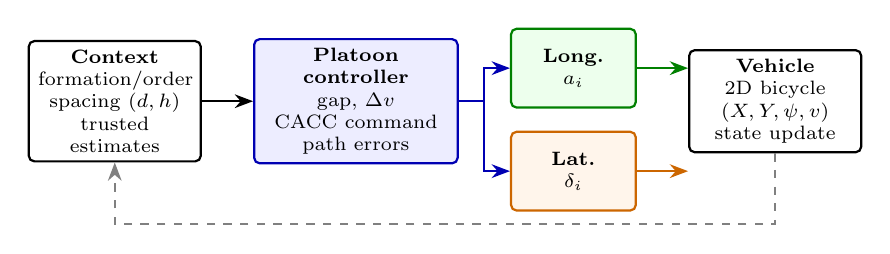
\begin{tikzpicture}[
        font=\scriptsize,
        >=Stealth,
        box/.style={draw, rounded corners=2pt, thick, align=center, minimum height=1.0cm, text width=1.95cm, fill=white},
        ctrl/.style={box, fill=blue!7, draw=blue!70!black, text width=2.35cm},
        cmd/.style={box, fill=green!7, draw=green!50!black, text width=1.35cm},
        lat/.style={box, fill=orange!8, draw=orange!80!black, text width=1.35cm},
        arrow/.style={->, thick},
        fb/.style={->, thick, dashed, gray}
    ]
        \node[box] (context) {
            \textbf{Context}\\
            formation/order\\
            spacing $(d,h)$\\
            trusted estimates
        };

        \node[ctrl, right=0.65cm of context] (controller) {
            \textbf{Platoon controller}\\
            gap, $\Delta v$\\
            CACC command\\
            path errors
        };

        \node[cmd, right=0.65cm of controller, yshift=0.42cm] (long) {
            \textbf{Long.}\\
            $a_i$
        };
        \node[lat, below=0.28cm of long] (lateral) {
            \textbf{Lat.}\\
            $\delta_i$
        };

        \node[box, right=0.65cm of long, yshift=-0.42cm] (vehicle) {
            \textbf{Vehicle}\\
            2D bicycle\\
            $(X,Y,\psi,v)$\\
            state update
        };

        \draw[arrow] (context) -- (controller);
        \draw[arrow, blue!70!black] (controller.east) -- ++(0.32,0) |- (long.west);
        \draw[arrow, blue!70!black] (controller.east) -- ++(0.32,0) |- (lateral.west);
        \draw[arrow, green!50!black] (long.east) -- (vehicle.west |- long.east);
        \draw[arrow, orange!80!black] (lateral.east) -- (vehicle.west |- lateral.east);
        \draw[fb] (vehicle.south) -- ++(0,-0.9cm) -| (context.south);
    \end{tikzpicture}}
    \caption{Compact vehicle-level controller for the QCar/LIMO rollback validation. The longitudinal command $a_i$ and lateral command $\delta_i$ are applied to the vehicle represented by the 2D kinematic bicycle model.}
    \label{fig:qcar_limo_vehicle_structure}
\end{figure}

The platform validation focuses on rollback rather than deterministic RMSE ranking. Unlike the numerical simulator, the real vehicles have non-deterministic packet delays, asynchronous sensing, and execution jitter. These effects can allow corrupted packets to enter the observer before the trust score falls below the rejection threshold, so the relevant comparison is between the same platform run without rollback and with finite-window rollback enabled. In the rollback case, once the delayed trust decision identifies the corrupted source, the host replays the recent observer window using the corrected trusted-neighbor set. The resulting behavior should be interpreted as mitigation, not perfect attack rejection: rollback improves the estimate after delayed detection, but the CACC-only controller may already have reacted to contaminated states. This limitation motivates the mixed local/cooperative control structure introduced next.

The implementation also separates diagnostic clean-motion tests from realistic observer operation. A clean-motion replay can use the uncorrupted heading and speed to propagate~\eqref{eq_pose_propagation}, but it keeps the estimator's current base position and therefore exposes residual pose contamination. A hard re-anchor according to~\eqref{eq_relative_pose_anchor}--\eqref{eq_pose_reanchor_prediction} is realistic only when the host has an accepted onboard relative measurement to the target, or another independently validated pose source. Re-anchoring to a clean reference channel that bypasses the attack injector is therefore used only as an ablation or debugging mode, not as evidence that the deployed observer has access to ground truth during an attack.

% Add QCar/LIMO rollback result figures here after the real-vehicle runs.
% Suggested figure 1: no-rollback versus rollback estimation error around the delayed detection time.
% Suggested figure 2: trust score, rollback trigger time, and corrected estimate trajectory.
% \begin{figure}[!t]
%     \centering
%     \includegraphics[width=\linewidth]{fig/qcar_limo_rollback_comparison.png}
%     \caption{QCar/LIMO rollback comparison under non-deterministic real-vehicle delay. The no-rollback case preserves the contaminated update, while rollback replays the recent observer window after the corrupted source is rejected.}
%     \label{fig:qcar_limo_rollback_comparison}
% \end{figure}

To make the platform results easier to inspect and reproduce, the QCar/LIMO source code and experimental resources used in this study are openly available at \url{https://github.com/kslhuy/QCar2_Cran}. An accompanying rollback-estimation demonstration video is provided at \url{https://youtu.be/t6-soznp6ks}.

\subsection{Distributed State Estimation for Platoon Control}
The proposed trust scores are useful at two levels. In the observer, they adapt the fusion weights so that unreliable V2V data have limited influence on the fleet-state estimate. In the controller, the same reliability information can gate how much the vehicle relies on cooperative CACC. This second use is important for safety: even after trust-aware estimation and rollback, a corrupted distributed estimate may still affect the command before a delayed trust decision is corrected. The longitudinal controller is therefore split into two channels: a local ACC channel based on direct sensing of the immediate predecessor, and a cooperative CACC channel based on the distributed estimates of the platoon. A trust gate fuses the two commands, so cooperation is used when the fleet estimate is credible and the controller falls back toward local ACC when it is not.

The planar bicycle states are first projected onto the road tangent,
\begin{align}
    e_{\parallel}(k)&=[\cos\psi_{\mathrm{ref}}(k),\sin\psi_{\mathrm{ref}}(k)]^\top,\\
    s_i(k)&=p_i(k)^\top e_{\parallel}(k),
\end{align}
where $p_i=[X_i,Y_i]^\top$. For follower $i\ge2$, let $\mathcal{P}_i=\{1,\ldots,i-1\}$ denote the set of predecessors used by the cooperative channel.

The closed-loop validation uses the worst numerical attack condition identified by the RMSE analysis. Let $i^\star$ denote the vehicle with the largest attack-window estimation degradation. Safety is checked through the minimum projected bumper-to-bumper spacing
\begin{equation}
    s_{\min}=\min_{k\in\mathcal{T}_{\mathrm{att}}}\min_{i=2,\ldots,N}
    \left((p_{i-1}(k)-p_i(k))^\top e_{\parallel}(k)-L\right).
\end{equation}
The tested interval is considered collision-free when $s_{\min}>0$.

The ACC branch is the local safety channel. Let $s_{i-1,i}(k)$ denote the projected bumper-to-bumper gap to the immediate predecessor obtained from onboard sensing. If direct sensing is unavailable, the same quantity may be built from an independently trusted relative measurement:
\begin{equation}
    s_{i-1,i}(k)
    =\big(r^{\mathrm{meas}}_{i,i-1}(k)\big)^\top e_{\parallel}(k)-L.
\end{equation}
The local constant-time-headway spacing target is
\begin{equation}
    s_{\mathrm{ACC},i}^{\star}(k)
    =d_{\mathrm{ACC}}+h_{\mathrm{ACC}}\max\{\hat{v}_0^{(i)}(k),0\}.
\end{equation}
Here $\hat v_0^{(i)}$ is vehicle $i$'s current ego-speed estimate from its local observer; the subscript $0$ denotes the local-observer channel, not a target vehicle.
The ideal ACC law uses only this local gap error:
\begin{align}
    e_{\mathrm{ACC},i}(k)
    &=s_{i-1,i}(k)-s_{\mathrm{ACC},i}^{\star}(k),\notag\\
    v_{\mathrm{ACC},i}^{\star}(k)
    &=v_{\mathrm{base},i}(k)+k_d e_{\mathrm{ACC},i}(k).
\end{align}
Thus, $v_{\mathrm{ACC},i}^{\star}$ is the ACC target speed. The low-level speed loop compares it with the current ego speed and maps the speed error to the local acceleration command,
\begin{equation}
    u_{\mathrm{loc},i}(k)
    =F_v\!\left(v_{\mathrm{ACC},i}^{\star}(k)-\hat v_0^{(i)}(k)\right),
\end{equation}
where $F_v$ denotes the speed controller. Saturation and emergency-stop limits are implementation details and are omitted here to keep the control structure clear. Because this branch does not use V2V estimates, it remains available when the cooperative channel is down-weighted.

The CACC branch is the cooperative performance channel. Host vehicle $i$ uses its distributed estimates $\hat p_i^{(j)}=[\hat X_i^{(j)},\hat Y_i^{(j)}]^\top$, $\hat v_i^{(j)}$, and $\hat\psi_i^{(j)}$ of each predecessor $j\in\mathcal{P}_i$. These estimates are compared with the host's local ego estimate $\hat p_0^{(i)}=[\hat X_0^{(i)},\hat Y_0^{(i)}]^\top$, $\hat v_0^{(i)}$, and $\hat\psi_0^{(i)}$:
\begin{align}
    u_{\mathrm{coop},i}
    &\equiv u_{\text{CACC},i}(k) \notag\\
    &= \sum_{j\in\mathcal{P}_i} \Big[
    \kappa_s e_{s,ij}(k)
    + \kappa_v e_{v,ij}(k)
    + \kappa_{\psi} e_{\psi,ij}(k)\Big],
\end{align}
where
\begin{align*}
    e_{s,ij}(k)&=\big(\hat p_i^{(j)}(k)-\hat p_0^{(i)}(k)\big)^\top e_{\parallel}(k)-d_{i,j}(k),\\
    e_{v,ij}(k)&=\hat{v}_i^{(j)}(k)-\hat{v}_0^{(i)}(k),\\
    e_{\psi,ij}(k)&=\mathrm{wrap}_{\pi}\big(\hat\psi_i^{(j)}(k)-\hat\psi_0^{(i)}(k)\big).
\end{align*}
Here $d_{i,j}(k)$ is the constant-time-headway spacing from vehicle $i$ to predecessor $j$; for a homogeneous platoon, $d_{i,j}(k)=(i-j)(d+h\hat{v}_0^{(i)}(k))$. The gains $\kappa_s$, $\kappa_v$, and $\kappa_{\psi}$ weight projected position, speed, and heading alignment.

The final acceleration command is obtained by trust fusion:
\begin{equation}
    u_{\text{target},i}(k)
    =u_{\mathrm{loc},i}(k)
    +\gamma_i(k)\big(u_{\mathrm{coop},i}(k)-u_{\mathrm{loc},i}(k)\big),
\end{equation}
where $\gamma_i(k)\in[0,1]$ is selected from the opinion vector defined in Section~\ref{sec_trust_score}. In the current implementation,
\begin{equation}
    \gamma_i(k)=\min_{j\in\mathcal{P}_i}\O_i(j,k).
\end{equation}
Thus, $\gamma_i=1$ recovers the cooperative CACC command, whereas $\gamma_i=0$ gives the local ACC fallback. The minimum operator is conservative: one low-trust predecessor is sufficient to reduce the cooperative contribution. A first-order filter smooths the applied command,
\begin{equation}
    u_i(k)=u_i(k-1)+\tau_f\big(u_{\text{target},i}(k)-u_i(k-1)\big),
\end{equation}
where $\tau_f\in[0,1]$ is the filter gain. The fusion controller should therefore be viewed as a safety-oriented use of the resilient estimator: improved fleet estimation supports cooperation, while local ACC limits the effect of unreliable distributed information. The present validation checks spacing preservation during the tested attack interval; a complete string-stability proof is left for future work.

% Add the closed-loop control figure/table here after running the physical or high-fidelity closed-loop test.
% Suggested report: worst attack case, most affected vehicle i^\star, minimum spacing s_min,
% spacing trajectory, and whether any inter-vehicle distance becomes non-positive.

\section{Discussion and Limitations}\label{sec_discussion}
The proposed method is designed to protect the platoon estimate and controller from unreliable incoming data, not to perform forensic reconstruction of a compromised vehicle. Once a neighbor is rejected by the trust layer, its information is no longer used as a cooperative correction source; accurate reconstruction of that vehicle then requires either a trusted independent measurement, a reliable local anchor, or a separate attack-identification module.

The ISS result also depends on bounded disturbances, bounded input mismatch, and sufficient trusted connectivity over time. If an attack removes all reliable paths to a target vehicle, no distributed observer can recover that target state from communication alone. Similarly, the rollback module improves delayed-decision recovery only when the required packets and weights remain inside the finite buffer and when trust-triggered resets do not occur arbitrarily fast. The current closed-loop evidence is limited to spacing preservation during the attack interval; string stability, sparse-topology operation, coordinated attacks, Monte Carlo noise/dropout behavior, and sensitivity to trust parameters require deeper validation.

\section{Conclusion and Future Work}\label{sec_conclusion}
This paper presented a trust-aware distributed observer for resilient state estimation in connected vehicle platoons. The proposed architecture combines local observer anchoring, distributed observer consensus, online trust evaluation, and an optional rollback module for delayed trust decisions. The trust scores define a time-varying trusted-neighbor set used directly in the observer-weight design, and sufficient ISS conditions were stated for bounded disturbances, input mismatch, and trust-induced switching. The evaluation is organized as a five-vehicle numerical RMSE campaign, a QCar/LIMO rollback validation for non-deterministic real-vehicle delays, and an estimation-based control check. Simulations under multiple attack cases show that the method can identify unreliable data and preserve bounded estimation errors. In the tested closed-loop scenario, the trust-modulated ACC/CACC controller preserves positive spacing during the attack interval.

Future work will focus on a deeper string-stability study of the closed loop, broader Monte Carlo validation, matrix-valued trust weights for channel-wise attack isolation, tighter dwell-time and contraction conditions for rollback-triggered resets, and stronger coupling between trust and control under dynamic communication topologies. Extending the QCar/LIMO validation to larger fleets and richer vehicle models is also a natural next step.

\bibliographystyle{IEEEtran}
\bibliography{biblio}
\end{document}
